% -*-coding: latin-9;-*-

%% To deal with the colors and number of slides per page according to the
%% \VersionPapier switch :
\ifx\VersionExpose\UnTrucInexistant%
% The handout version
\documentclass[aspectratio=169,handout,compress,10pt,hyperref={hyperindex},xcolor={svgnames,x11names}]{beamer}
\usepackage{pgfpages}
\pgfpagesuselayout{4 on 1}[a4paper,landscape,border shrink=5mm]
\else
% The slide version
\documentclass[aspectratio=169,compress,10pt,hyperref={hyperindex},xcolor={svgnames,x11names}]{beamer}
\fi

\usepackage[latin9]{inputenc}

% Local definitions to this course:
%\usepackage{header_cours_hpc_project-here}
\usepackage{header_SYCL}

% Some specialization according to the official Xilinx 2018 PowerPoint
% template
\usepackage{beamer_RK}

% To add arrows between slide pieces:
% Here because of catcode wizardy I guess :-(
% Should go into tikz_hpc
% Could use \pgftext instead of using "text depth=0pt"
\newcommand{\PlaceTextNode}[2]{\tikz{\node[inner sep=0pt,text depth=0pt] (#1) {#2};}}

% To decorate some lstlisting lines:
\usepackage{balloon_rk}


\author[]{Ronan Keryell (\url{rkeryell@xilinx.com})}

\title{SYCL: a programming standard for heterogeneous computing based on
modern C++}

%\subtitle{From single-source modern C++ down to FPGA}

\date{\href{https://www.meetup.com/ACCU-Bay-Area/events/264402705}
  {2019/10/09 @ Association of C and C++ Users - San Francisco Bay Area}}

\institute[]{Khronos Group \& Xilinx Research Labs, San Jos�, California}


\pgfdeclareimage[width=0.8cm]{logo-SYCL}{Khronos/Logos/SYCL/SYCL_500px_June16}
\logo{\hbox to 0.75cm{\vbox{%
      \href{https://www.khronos.org/sycl}{\pgfuseimage{logo-SYCL}}}}}


% Use SYCL+OpenCL as the default language
\lstset{language=SYCL,showstringspaces=false,
  basicstyle=\small}

\begin{document}

{
  % A background adapted from the official PowerPoint template
  \SetImageBackground{Background/Khronos-background-16-9}

  \begin{frame}[plain]
%\tracingall=1
    \titlepage
%\tracingall=0
  \end{frame}
}

\section{The Zoo}

\begin{frame}{Power wall \& speed of light: the final frontier...}
  \begin{itemize}
  \item Current physical limits
    \begin{itemize}
    \item Power consumption
      \begin{itemize}
      \item Cannot power-on all the transistors without melting
        (\vavers \emph{dark silicon})
      \item Accessing memory consumes orders of magnitude more energy
        than a simple computation
      \item Moving data inside a chip costs quite more than a
        computation
      \end{itemize}
    \item Speed of light
      \begin{itemize}
      \item Accessing memory takes the time of $10^4$+ CPU instructions
      \item Even moving data across the chip (cache) is slow at 1+ GHz...
      \end{itemize}
    \end{itemize}
  \end{itemize}
\end{frame}

%\end{document}

% openpowerfoundation.org/wp-content/uploads/2016/02/12_Ralph-Wittig.Xilinx.pdf
\begin{frame}[fragile]{(Very old) 45nm technology characteristics}
  \relax
  {\scriptsize Tutorial on ``\emph{High-Performance Hardware for
      Machine Learning}'', William Dally at NIPS, December 7th, 2015
    \url{https://media.nips.cc/Conferences/2015/tutorialslides/Dally-NIPS-Tutorial-2015.pdf}}
  \\[-7mm]


  \centerline{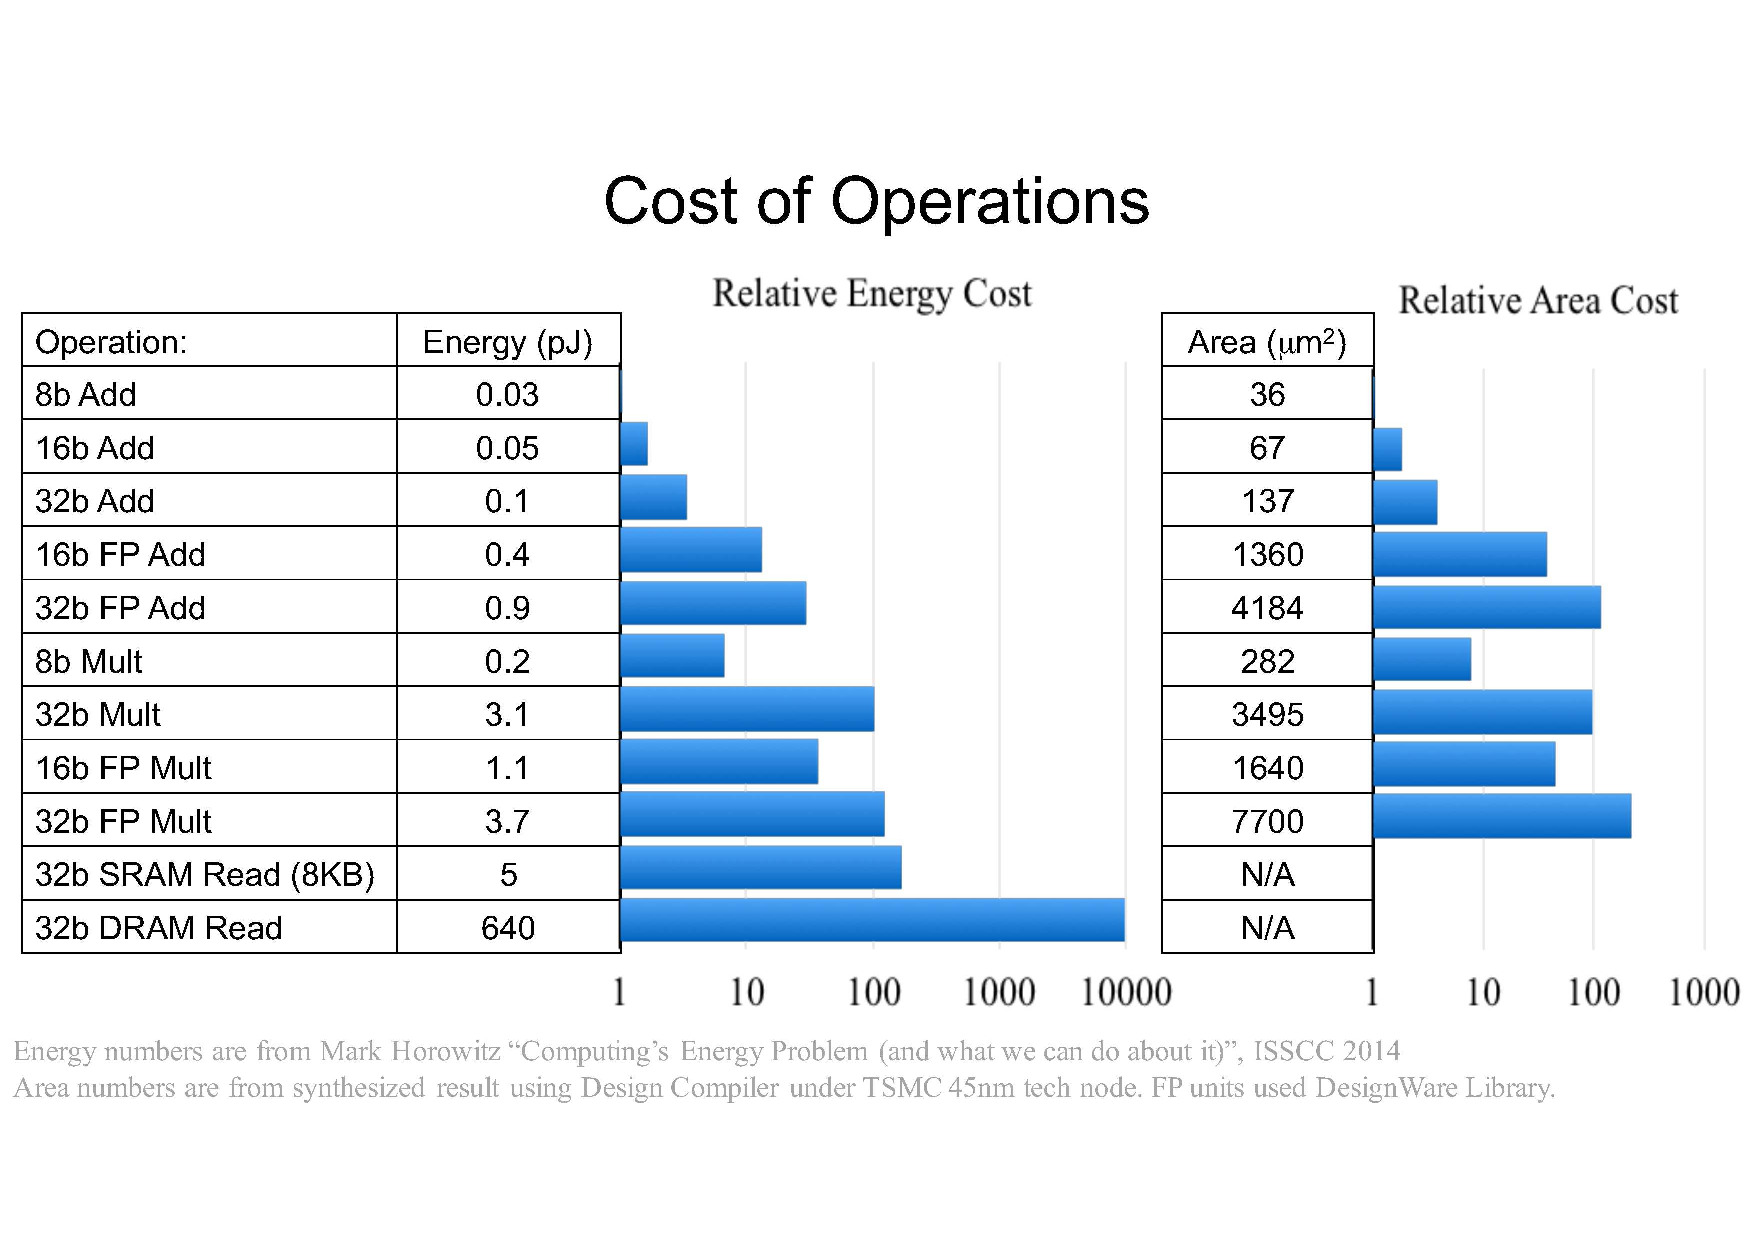
\includegraphics[height=0.95\textheight]{Technology/IC/NIPS_Tutorial_Final-p57-energy-area}}
\end{frame}


\begin{frame}[fragile]{Space-time traveling}
  \relax
  % http://hps.ece.utexas.edu/yale75/dally_slides.pdf
  % http://www.cs.colostate.edu/~cs575dl/Sp2015/Lectures/Dally2015.pdf slide 45 which looks nice.
  {\scriptsize ``\emph{Challenges for Future Computing Systems}'',
    William J. Dally, January 19, 2015, HiPEAC 2015.
    \url{http://www.cs.colostate.edu/~cs575dl/Sp2015/Lectures/Dally2015.pdf}}\\[-7mm]

  \centerline{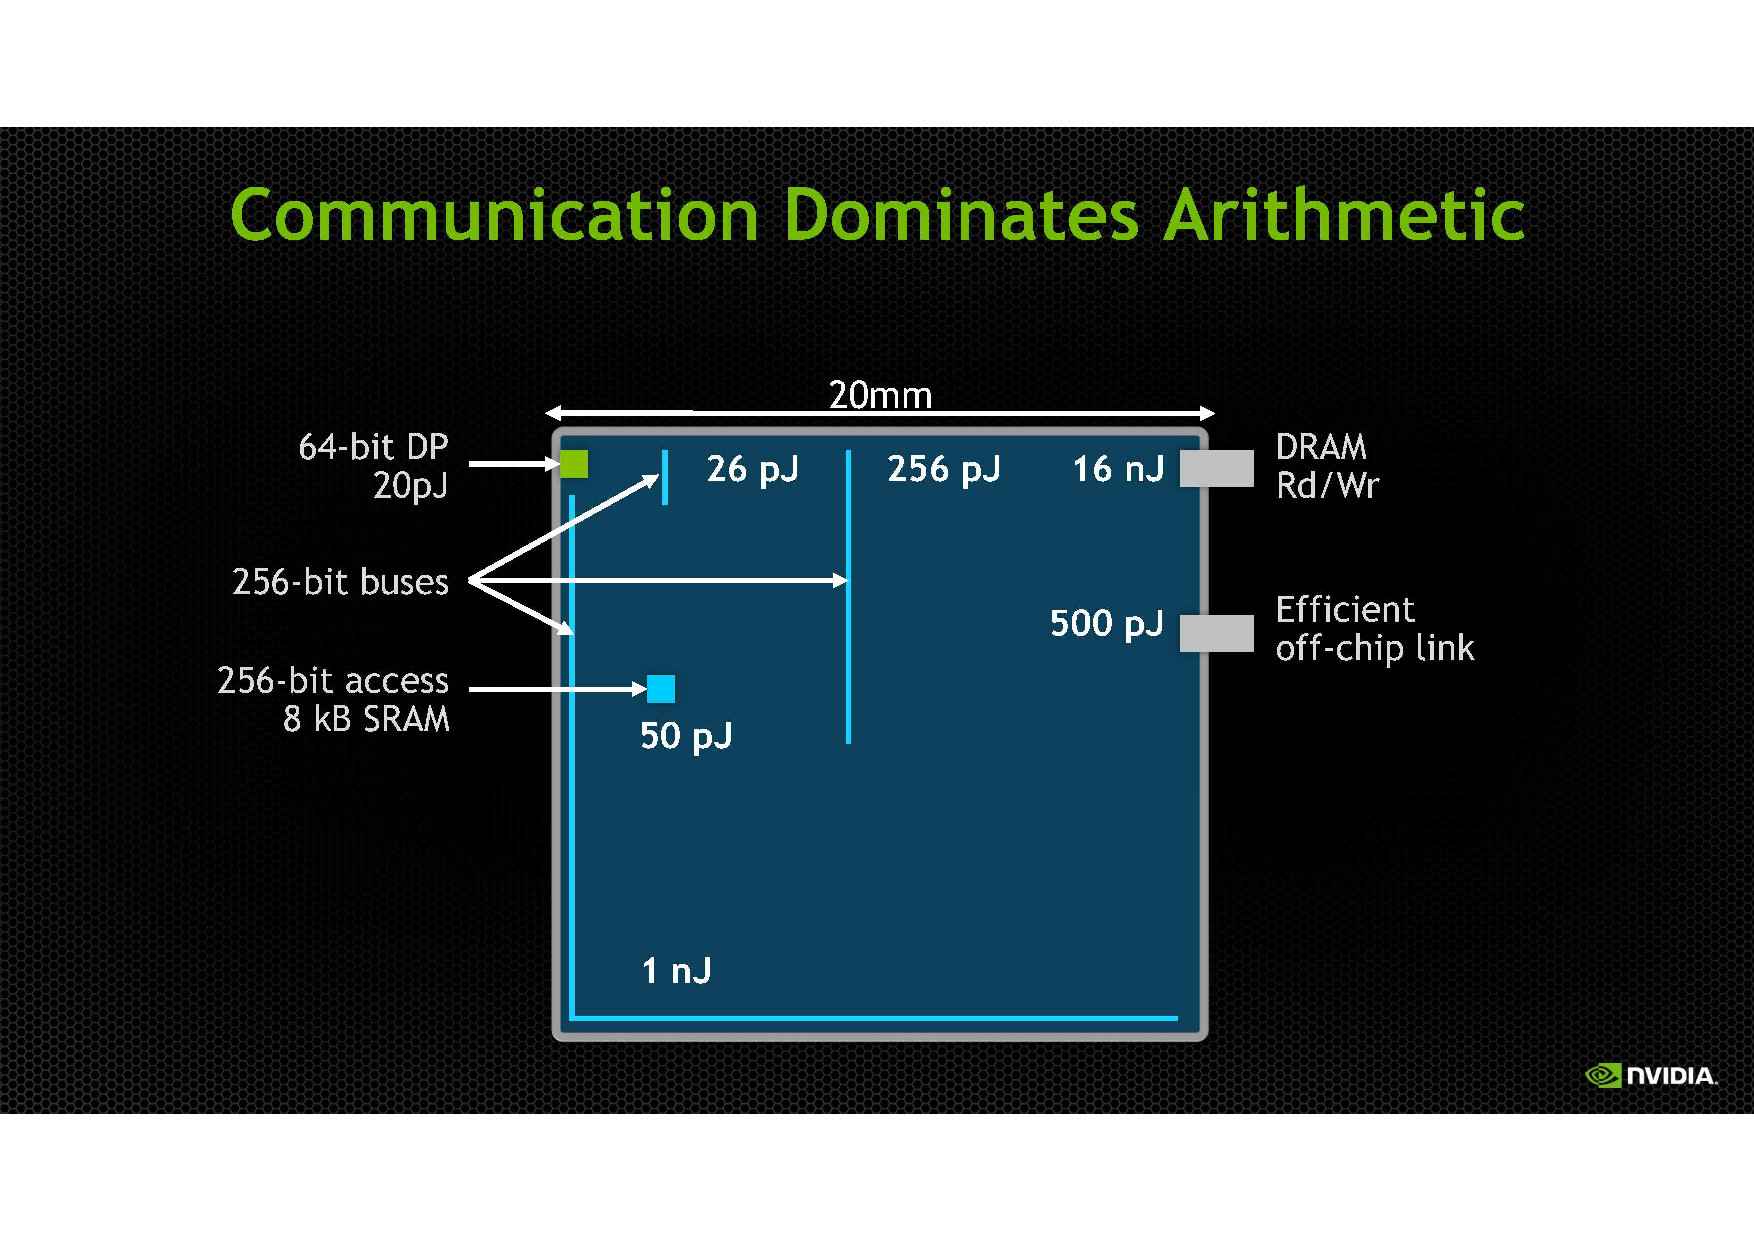
\includegraphics[height=0.95\textheight]{Technology/IC/Dally2015-p45-communication_arithmetic}}
\end{frame}


\begin{frame}{Power wall \& speed of light: implications}
  \begin{itemize}
  \item Change hardware and software
    \begin{itemize}
    \item Use locality \& hierarchy
    \item Massive parallelism
    \end{itemize}
  \item NUMA \& distributed memories
    \begin{itemize}
    \item \vavers New memory address spaces (local, constant, global,
      non-coherent...)
    \item \vavers PiM (Processor-in-Memory), Near-Memory Processing
      (in 3D memory stack controller)...
    \end{itemize}
  \item Specialize architecture
  \item Power on-demand only what is required
  \end{itemize}
  Nice take-away: the battery limitation may produce better
  programmers in the future \smiley
\end{frame}


\begin{frame}{ACM Turing award 2017: John L. Hennessy \& David A. Patterson}

  \begin{BoiteA}{\emph{A New Golden Age for Computer Architecture}}
    John L. Hennessy, David A. Patterson, Communications of the ACM,
    February 2019, Vol. 62 No. 2, Pages 48-60
  \end{BoiteA}
  \url{https://cacm.acm.org/magazines/2019/2/234352-a-new-golden-age-for-computer-architecture/fulltext}

  Award lecture: \url{https://www.youtube.com/watch?v=3LVeEjsn8Ts}

  \begin{itemize}
  \item \emph{``Those who cannot remember the past are condemned to
      repeat it''},\\
    George Santayana, 1905
  \item \emph{``What we have before us are some breathtaking opportunities
    disguised as insoluble problems''}, John Gardner, 1965
  \item \vavers{} Agile Hardware \& Software Development
    \begin{itemize}
    \item Open Architectures, inspired by the success of open
      source software
    \end{itemize}
  \end{itemize}

  \bigskip

  \begin{beamerboxesrounded}[scheme=bleuvert]{}
    \begin{quote}
      ``The next decade will see a Cambrian explosion of novel computer
      architectures, meaning exciting times for computer architects in
      academia and in industry.''
    \end{quote}
  \end{beamerboxesrounded}
\end{frame}


\begin{frame}{AMD 7nm ``Navi'' GPU @ HotChips-31 2019}
  \centerline{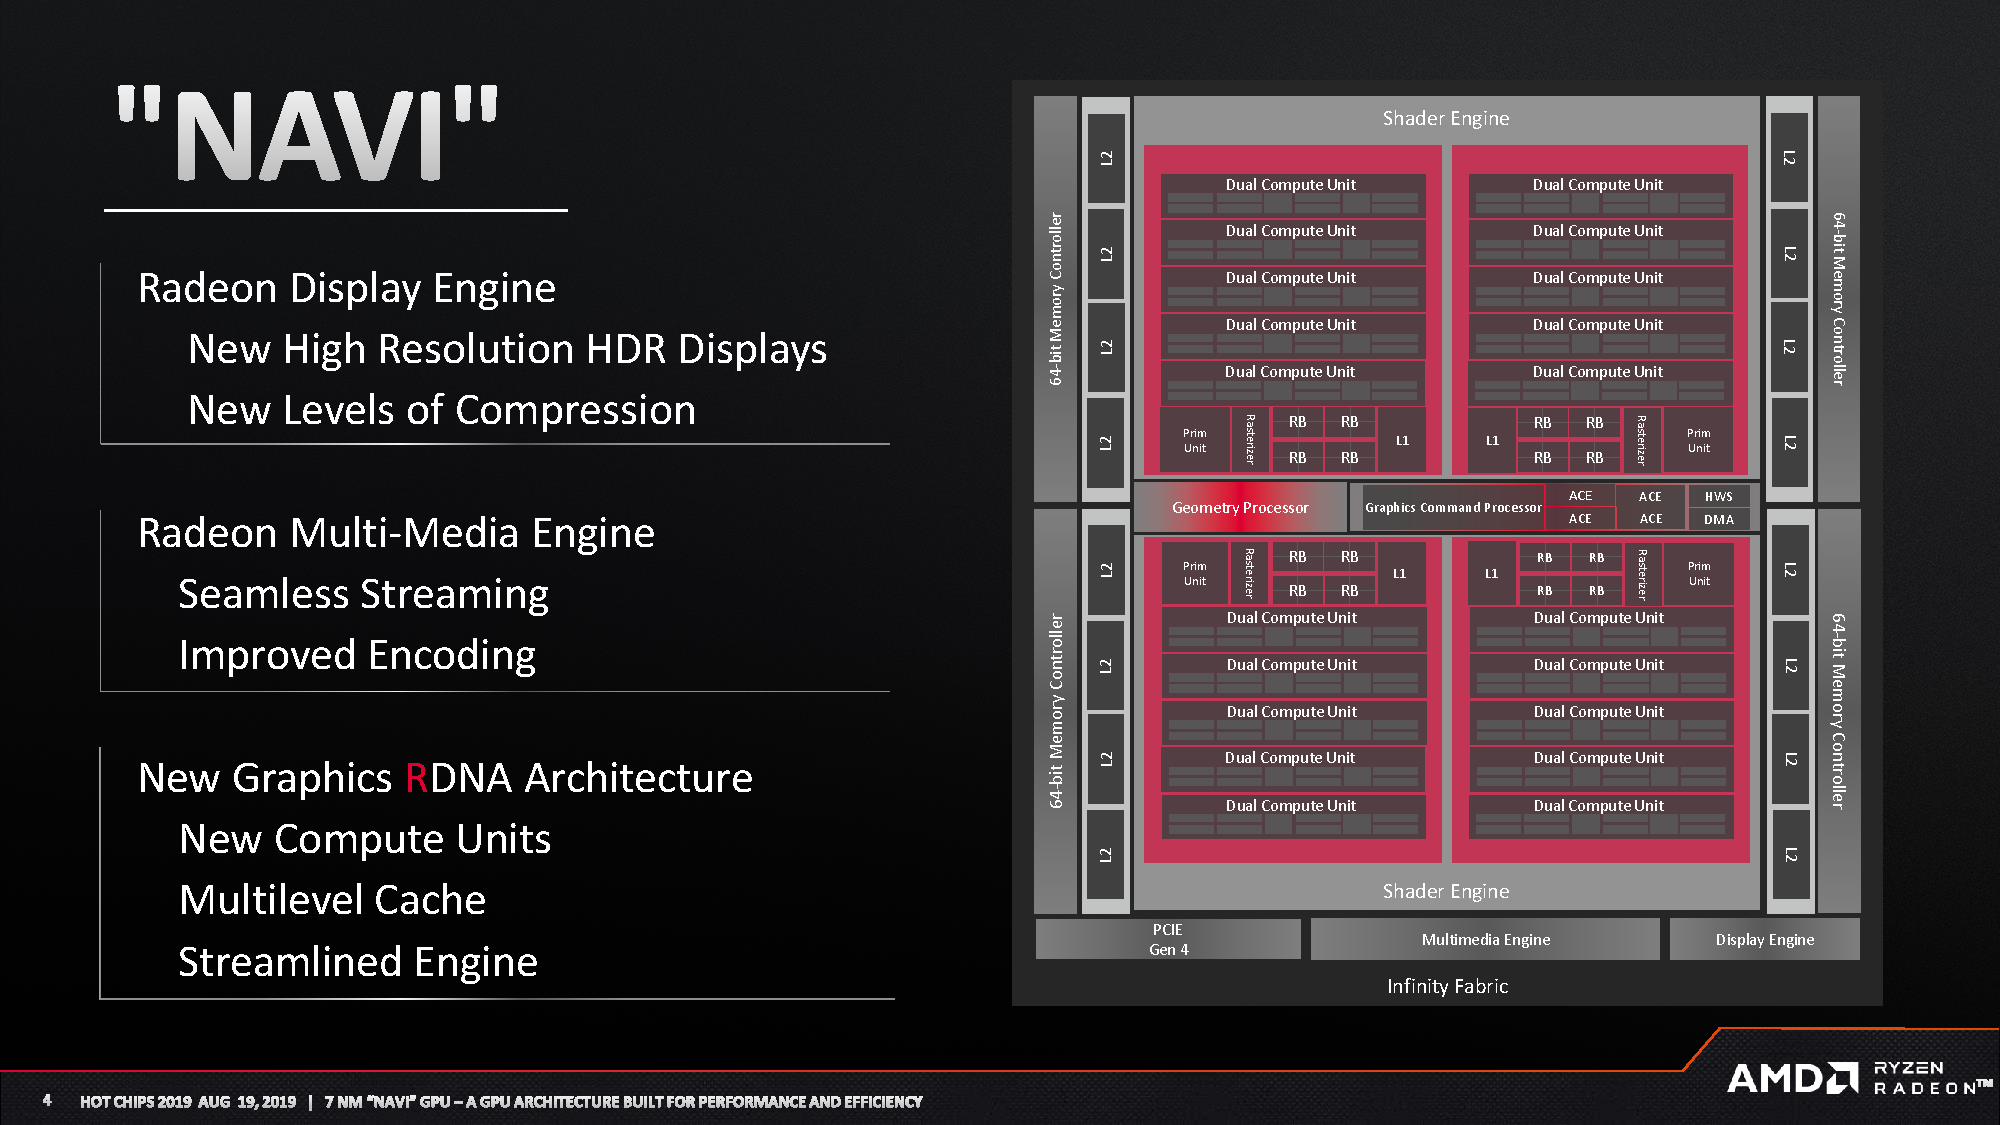
\includegraphics[height=0.91\vsize]{ordinateurs/AMD/GPU/Navi/HotChips-2019/HC31_2_13_AMD_final-slide4-high-level}}
\end{frame}


\begin{frame}{Nvidia Turing GPU @ HotChips-31 2019}
  \centerline{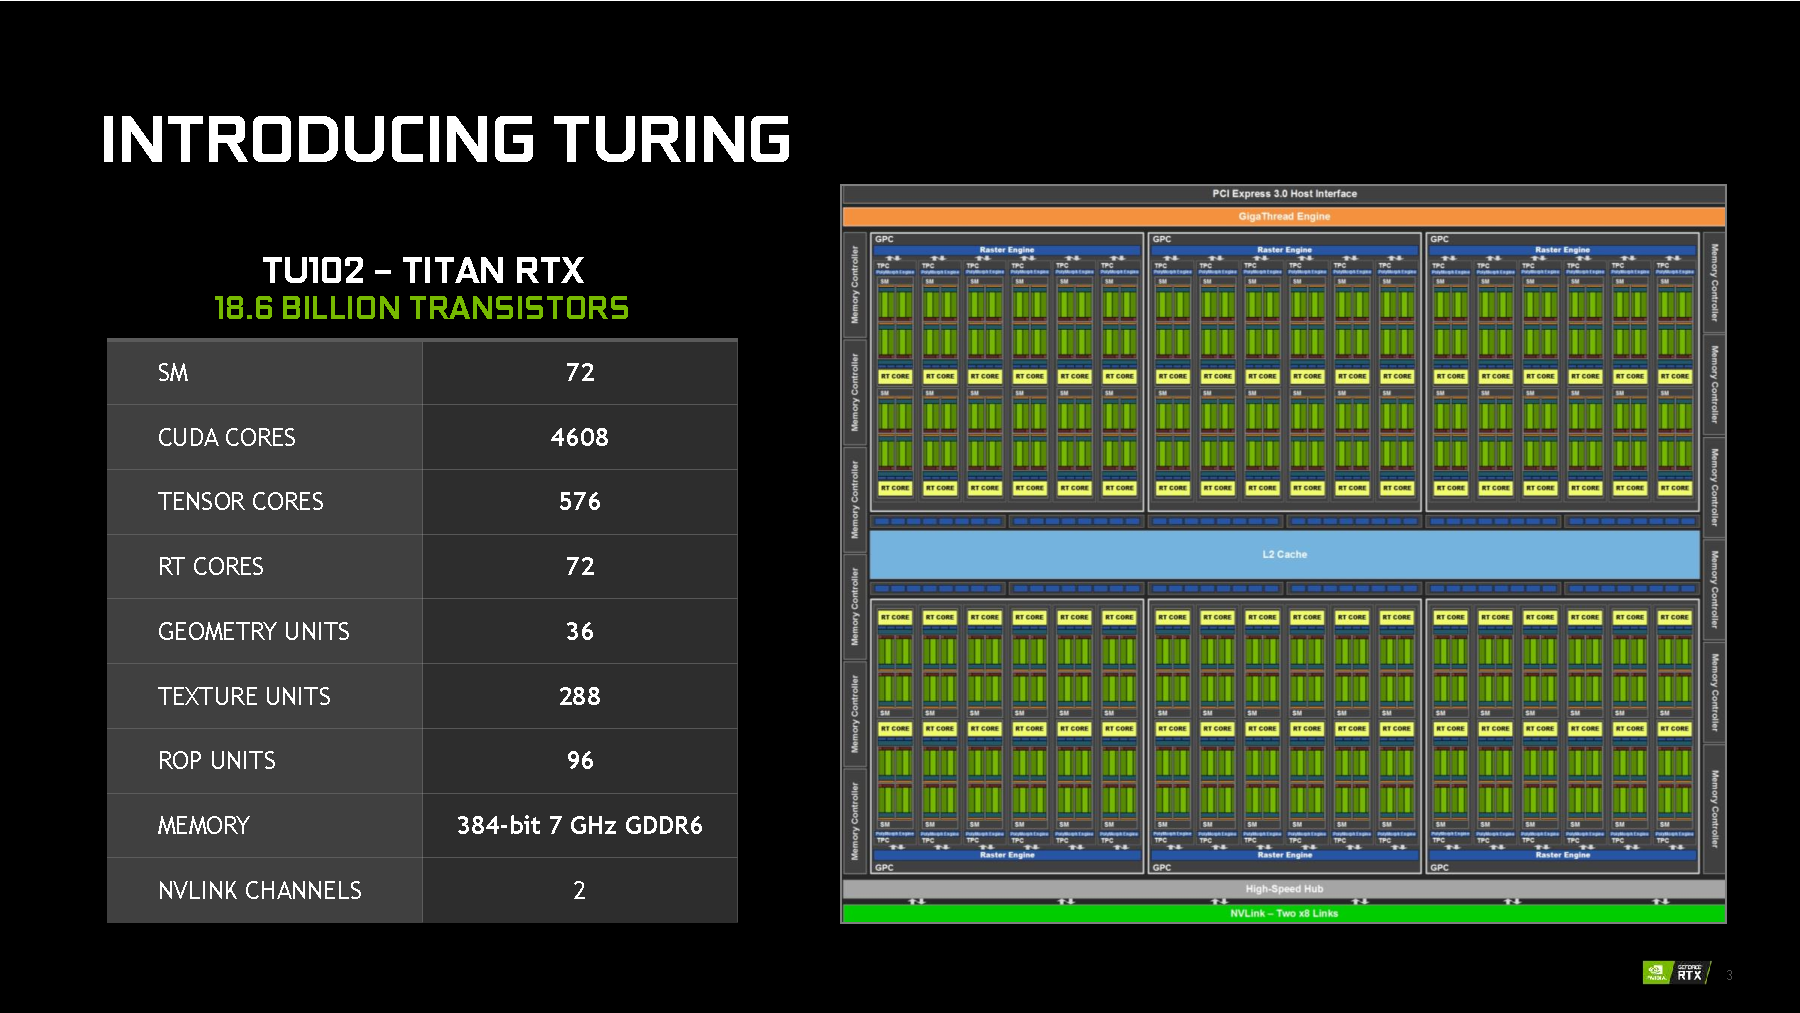
\includegraphics[height=0.9\vsize]{ordinateurs/nVidia/Turing/HotChips-2019/HC31_2_12_NVIDIA_final-slide3-introducing_Turing}}
\end{frame}


\begin{frame}
  \begin{center}
    \Huge
    But wait...

    \bigskip

    92\% of HotChips 2019 presentations are \alert{not about GPU}!
  \end{center}
\end{frame}


\begin{frame}{Tesla Neural Network Accelerator @ HotChips-31 2019}
  \centerline{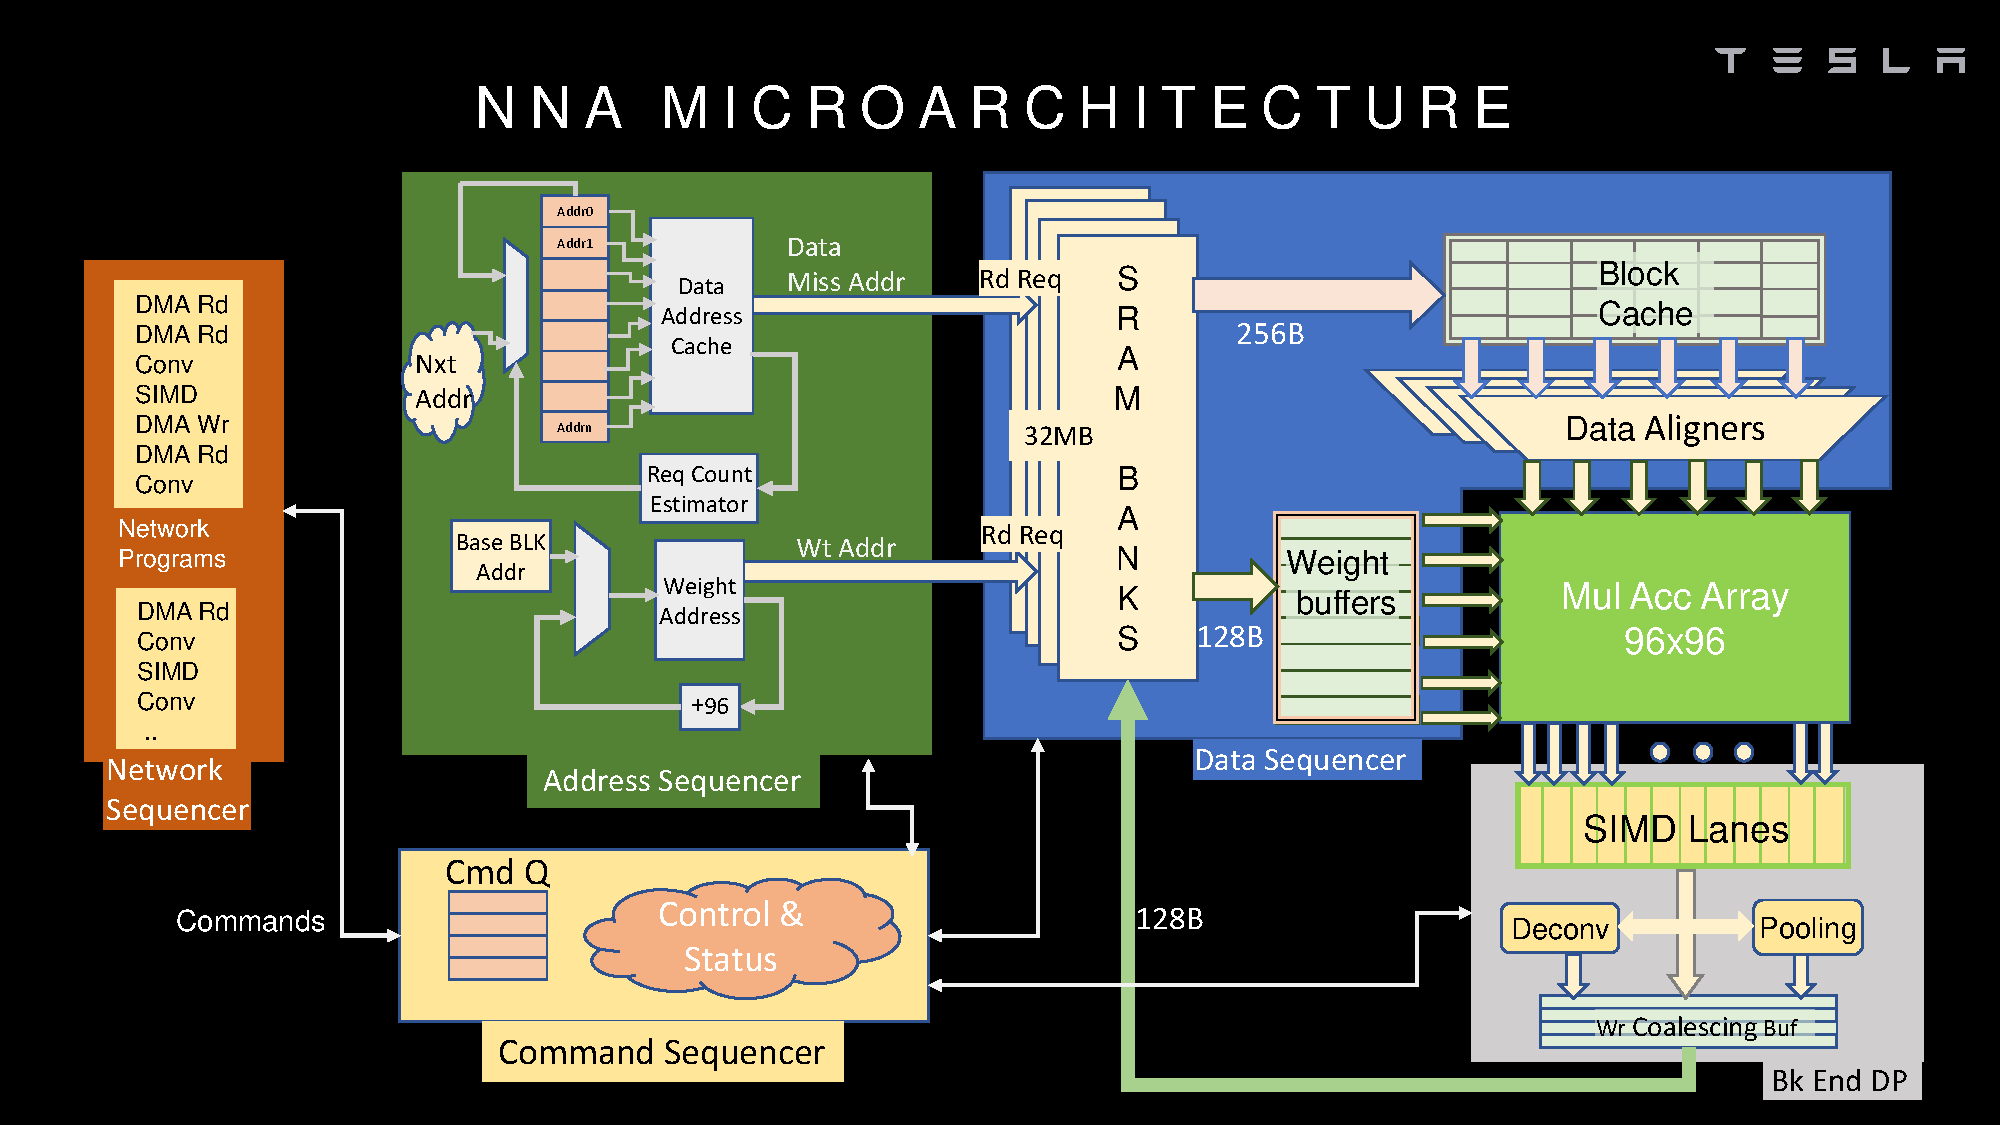
\includegraphics[height=0.9\vsize]{ordinateurs/Tesla/HotChips-2019/HC31_2_3_Tesla_Hotchips_ppt_Final_0817-slide16-NNA-microarchitecture}}
\end{frame}


\begin{frame}{Habana Gaudi Processor for training @ HotChips-31 2019}
  \centerline{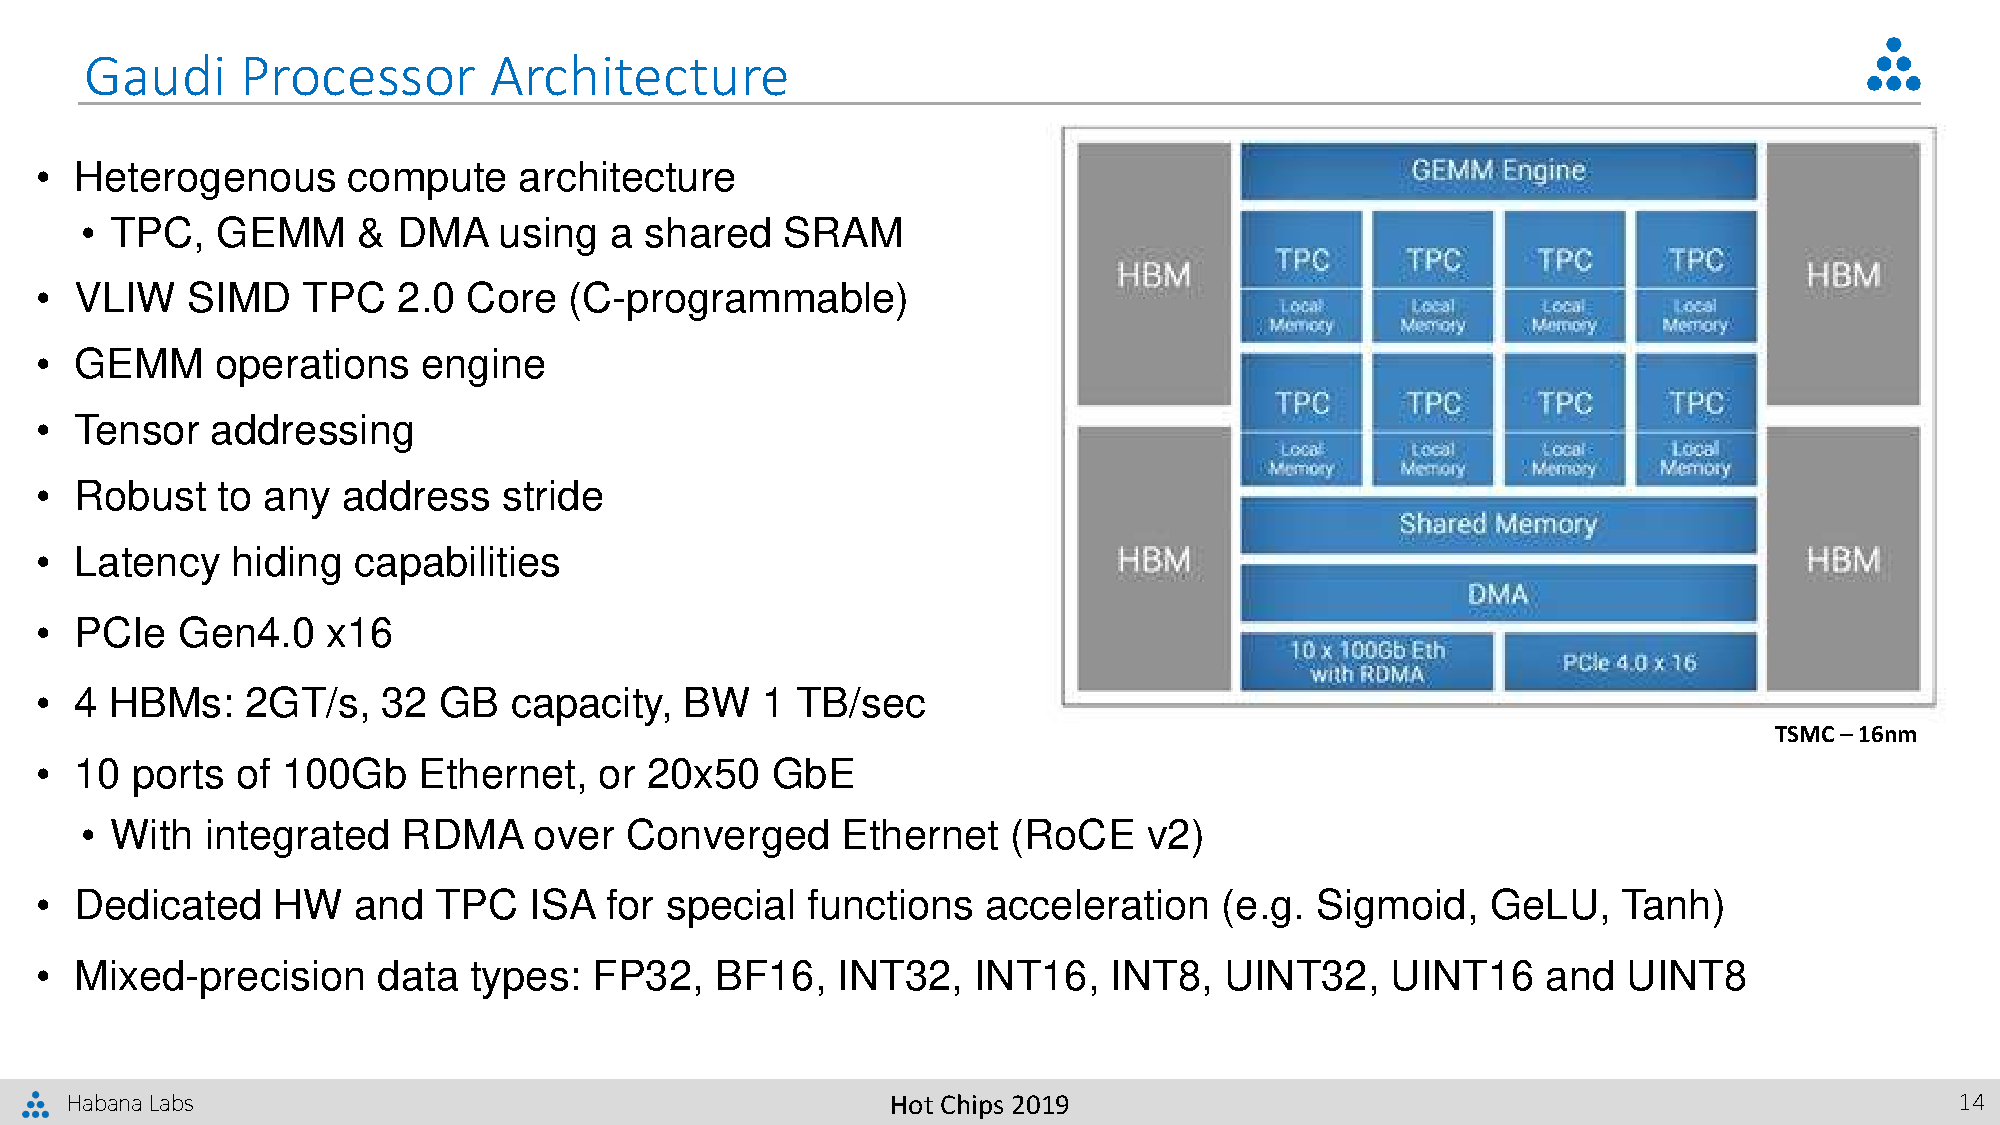
\includegraphics[height=0.9\vsize]{ordinateurs/Habana/HotChips-2019/HC31_1_14_HabanaLabs_Eitan_Medina_v9-slide14-Gaudi_Processor_Architecture}}
\end{frame}


\begin{frame}{Intel Nervana NNP-T for training @ HotChips-31 2019}
  \centerline{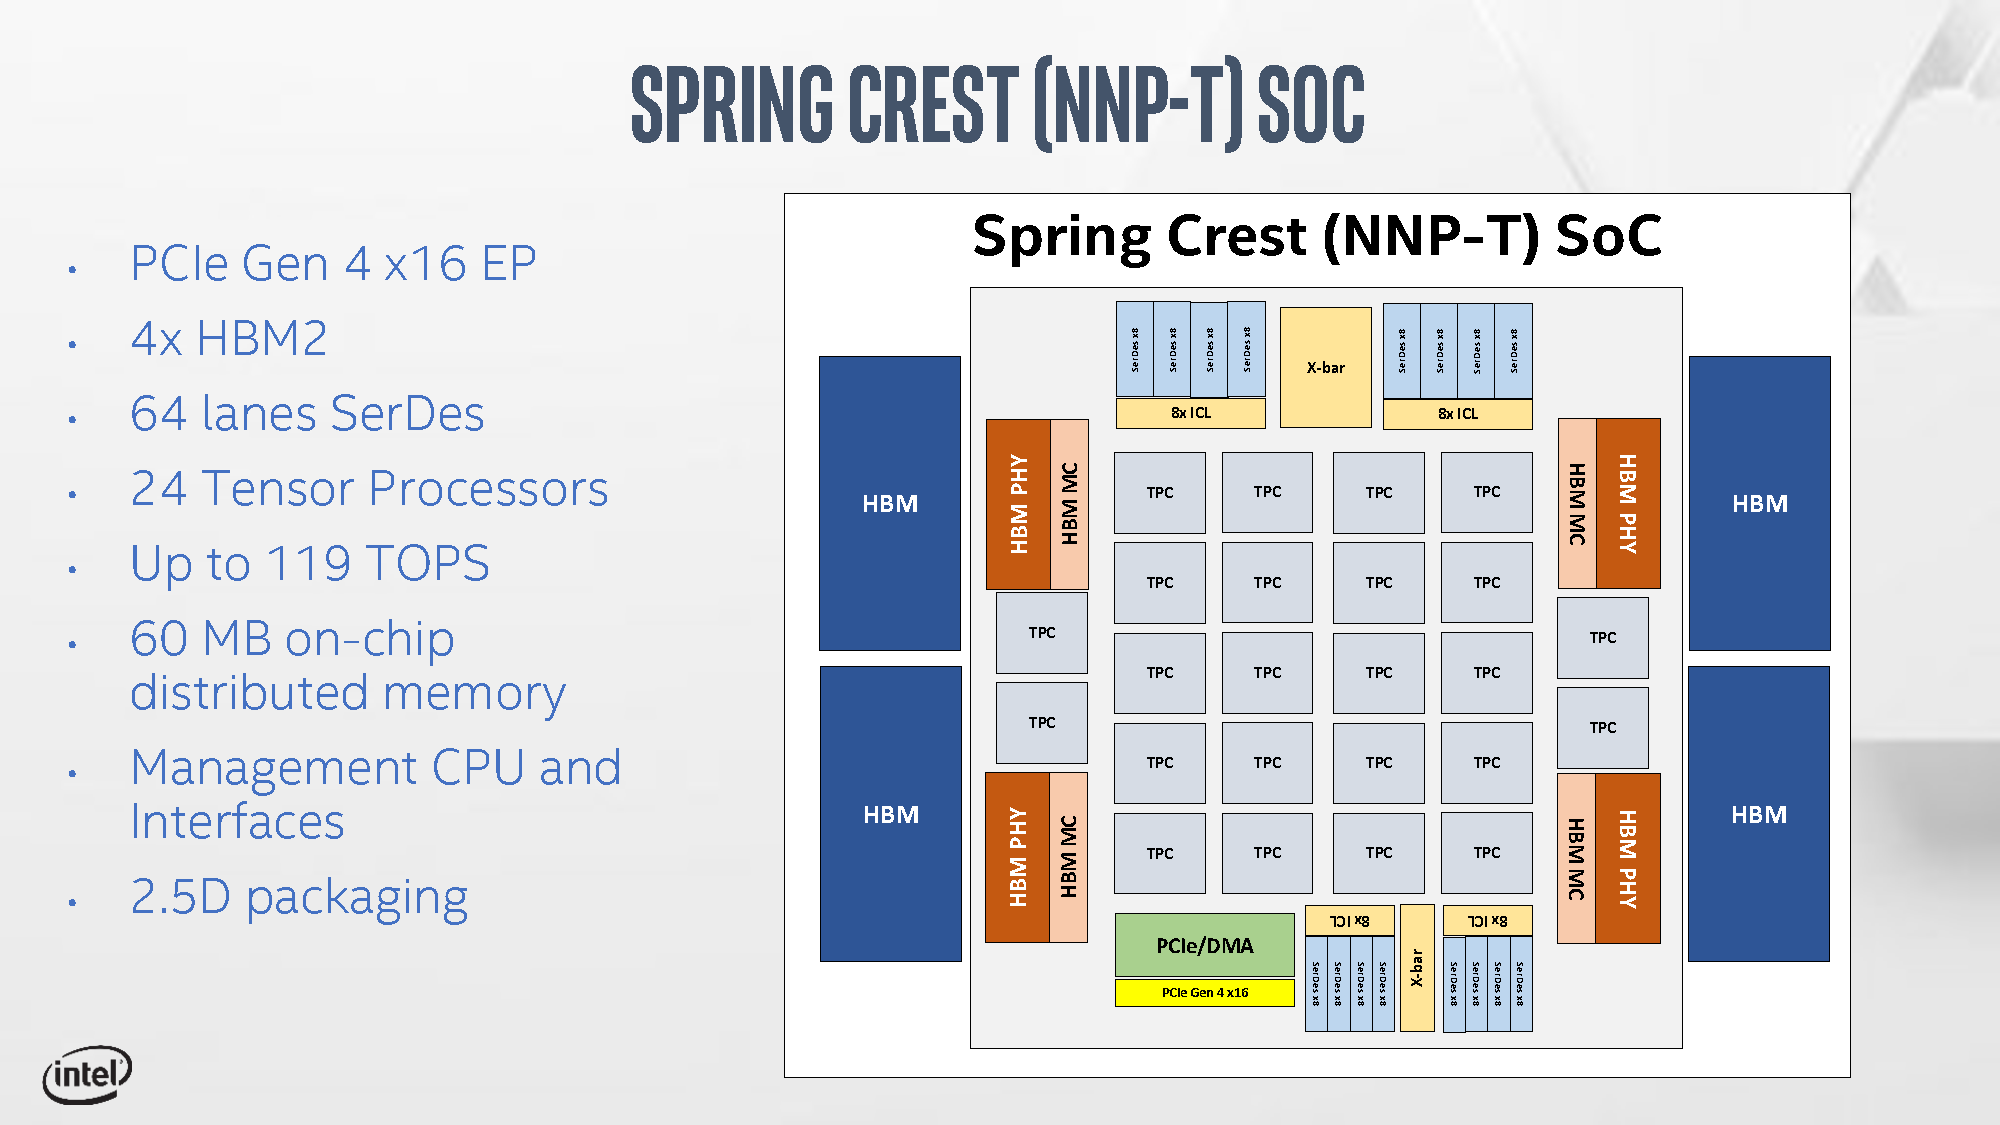
\includegraphics[height=0.9\vsize]{ordinateurs/Intel/Nervana/NNP-T/HotChips-2019/HC31_1_12_Intel_Intel_AndrewYang_v0_92-slide5-Spring_Crest_NNP-T_SoC}}
\end{frame}


\begin{frame}{Cerebras Wafer-Scale Deep Learning @ HotChips-31 2019}
  \centerline{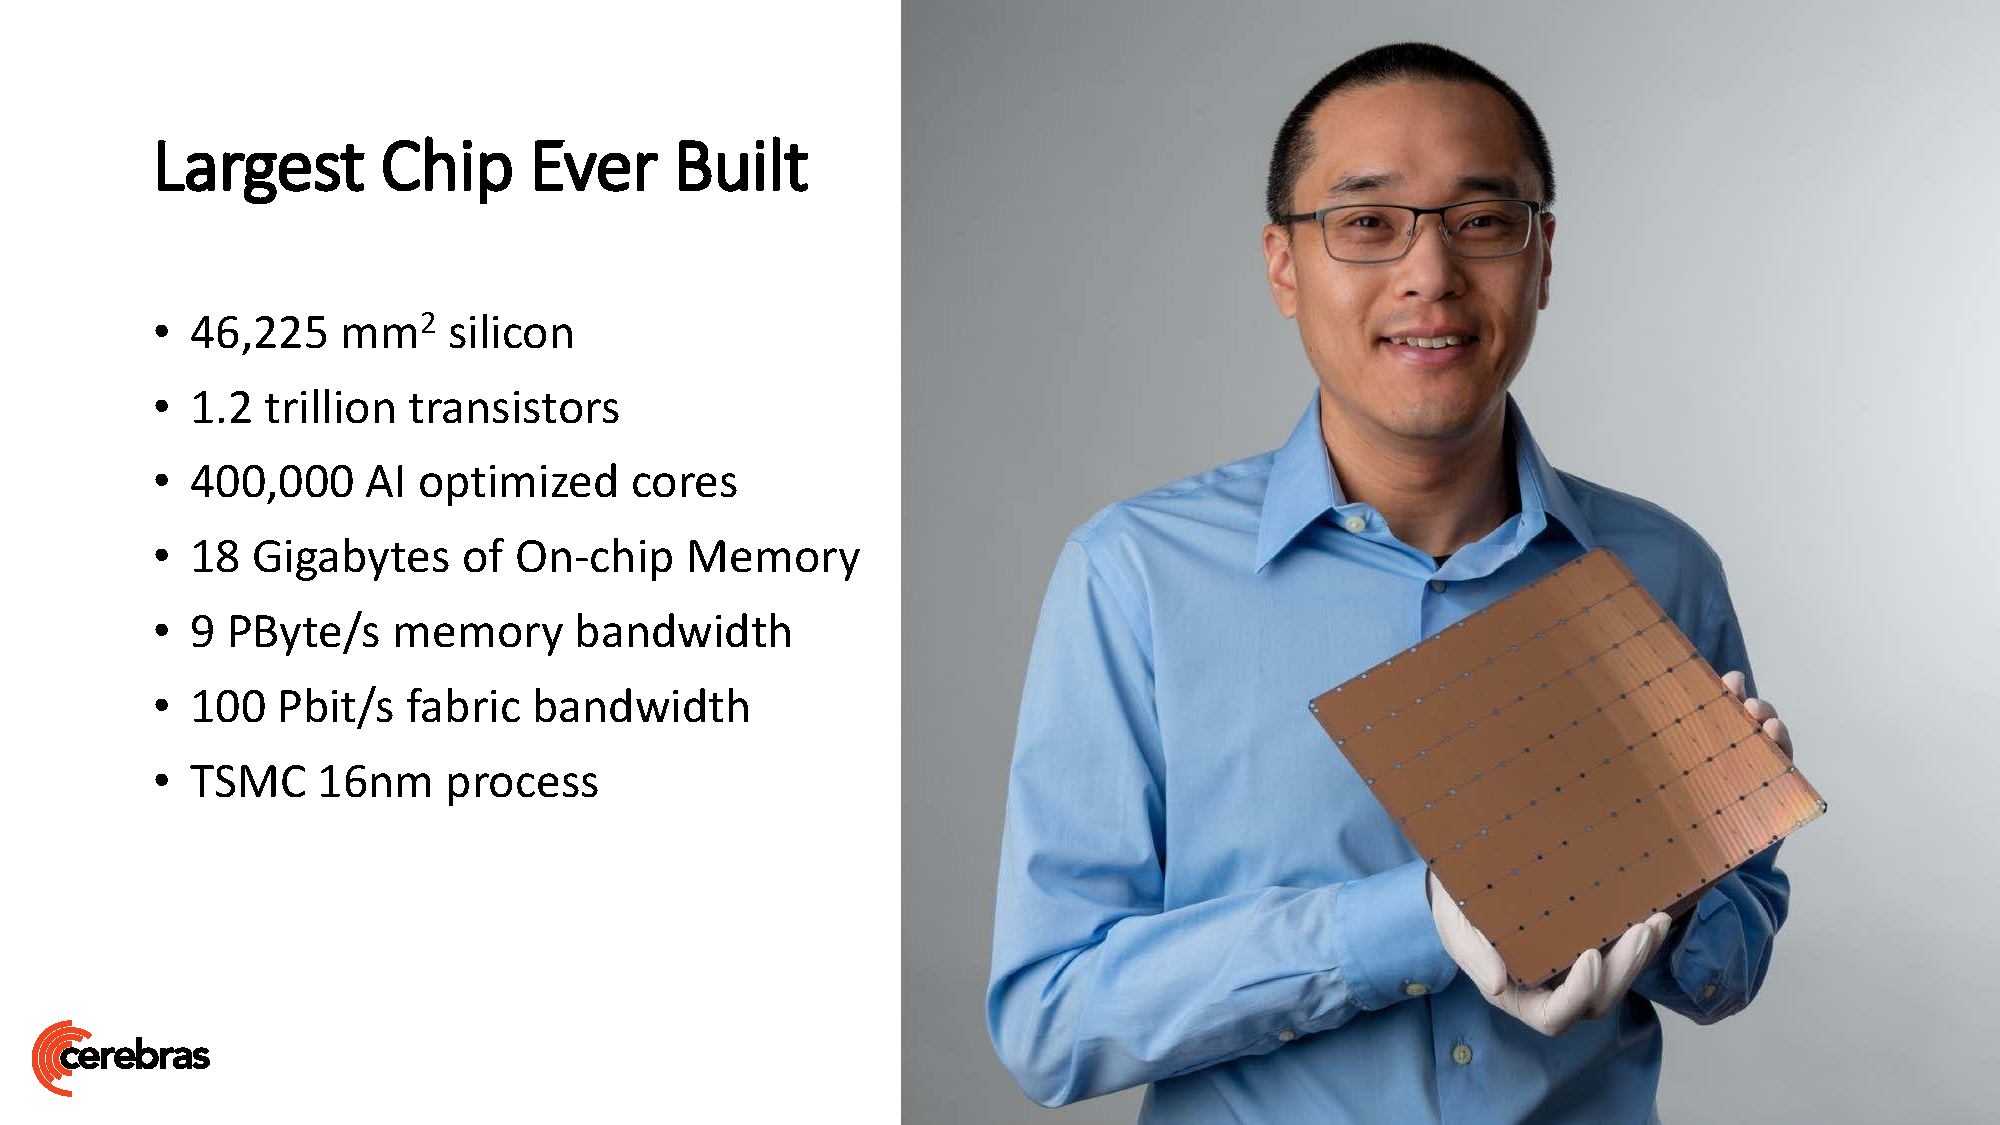
\includegraphics[height=0.9\vsize]{ordinateurs/Cerebras/HotChips-2019/HC31_1_13_Cerebras_SeanLie_v02-slide2-Largest_Chip_Ever_Built}}
\end{frame}


\begin{frame}{UPMEM: Processing In Memory accelerator @ HotChips-31
    2019}
  \centerline{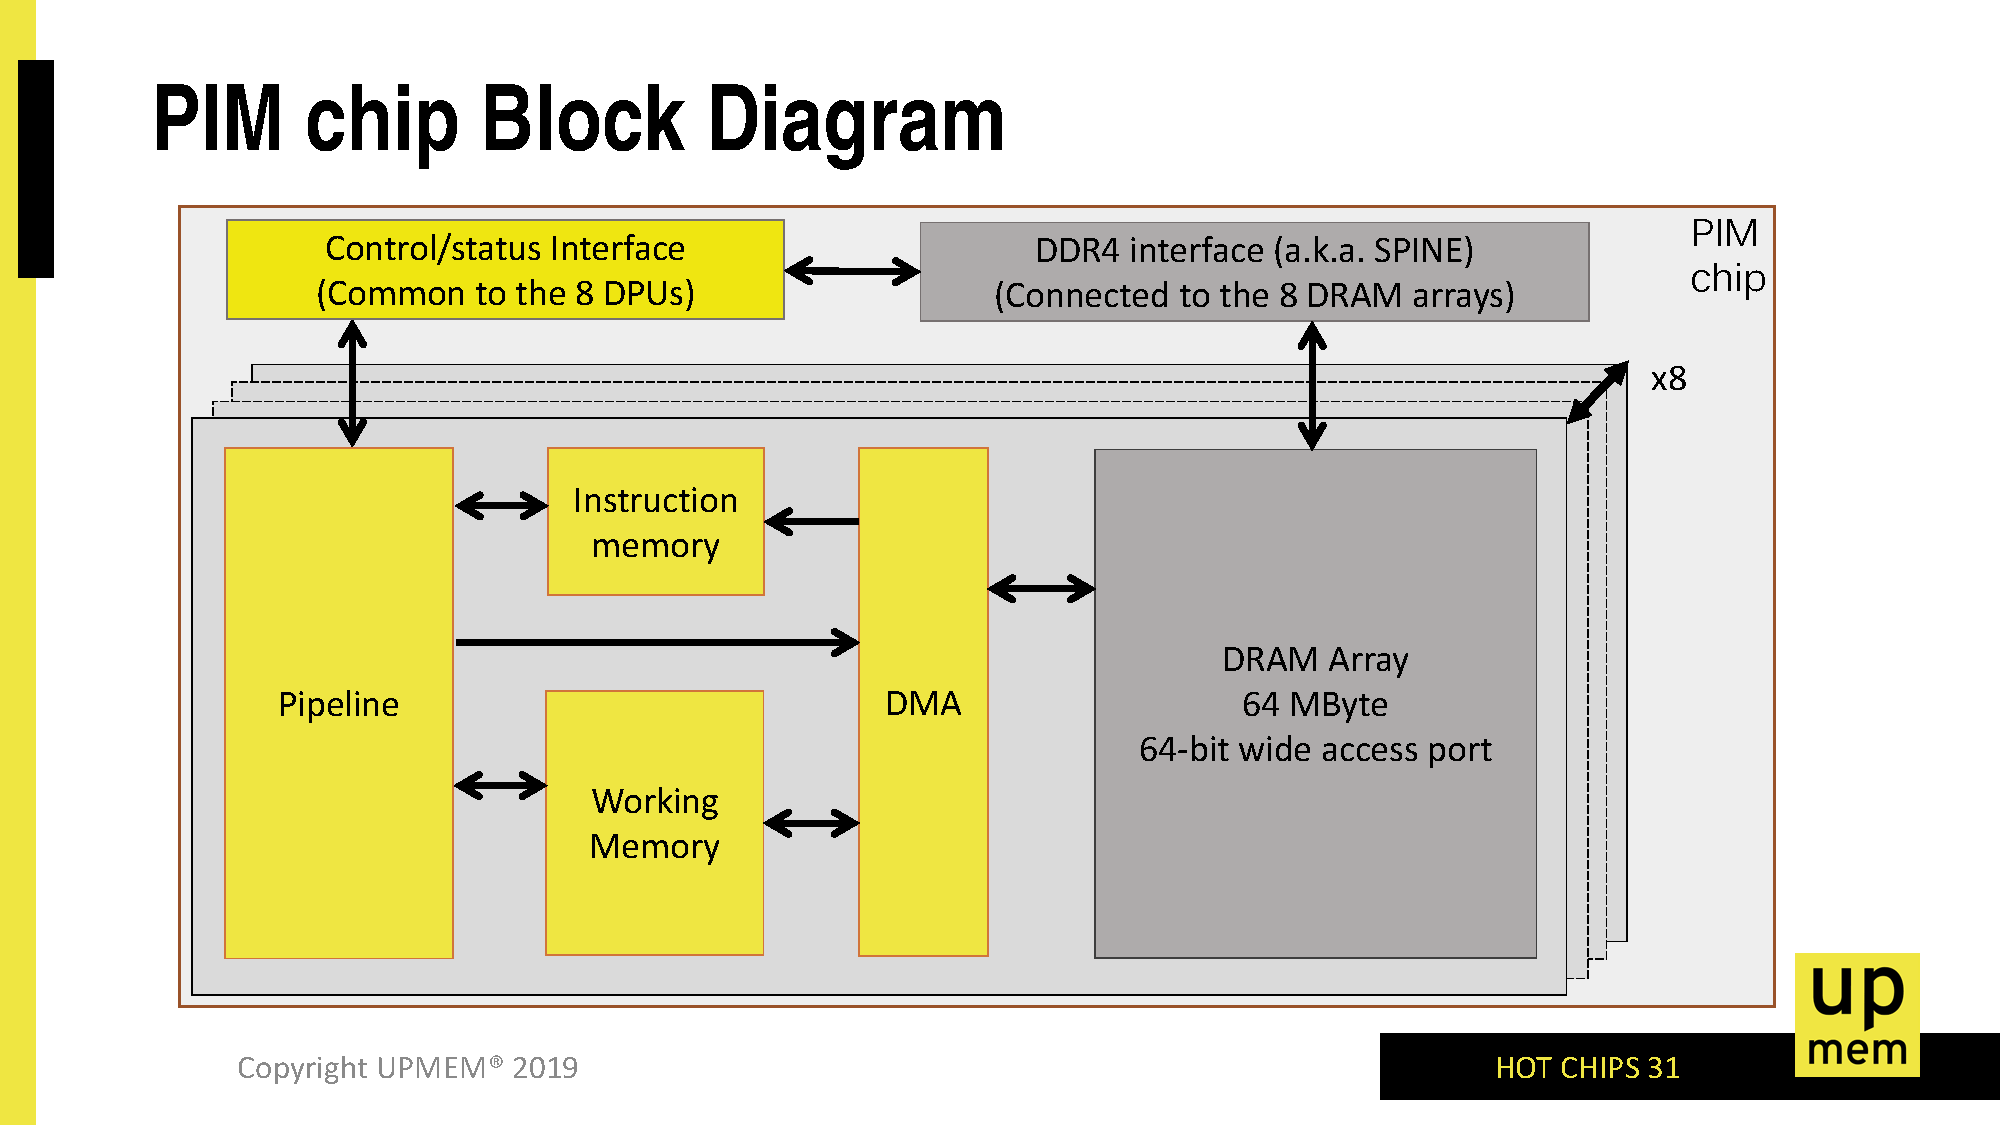
\includegraphics[height=0.9\vsize]{ordinateurs/UPmem/HotChips-2019/HC31_1_4_UPMEM_FabriceDevaux_v2_1-slide14-PIM_chip_Block_Diagram}}

  \begin{tikzpicture}[remember picture,overlay]
    \node [%xshift=-0.427\paperwidth,
    yshift=-0.1\paperheight,
    anchor=north east
    ]
    at (current page.north east)
    {
      \includegraphics[width=0.55\hsize]{ordinateurs/UPmem/HotChips-2019/HC31_1_4_UPMEM_FabriceDevaux_v2_1-slide5-DDIM-picture}
    };
  \end{tikzpicture}
\end{frame}


\begin{frame}{Deconstructivism in (hardware) architecture: FPGA}
  \centerline{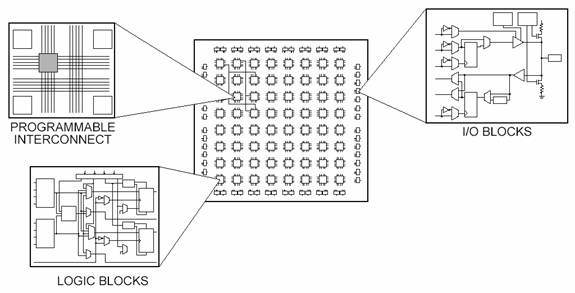
\includegraphics[height=0.5\textheight]{Images/Xilinx/FPGA/FPGA-main-qimg-f34b651c2753c3165acef62a9ab19e6e-c}
    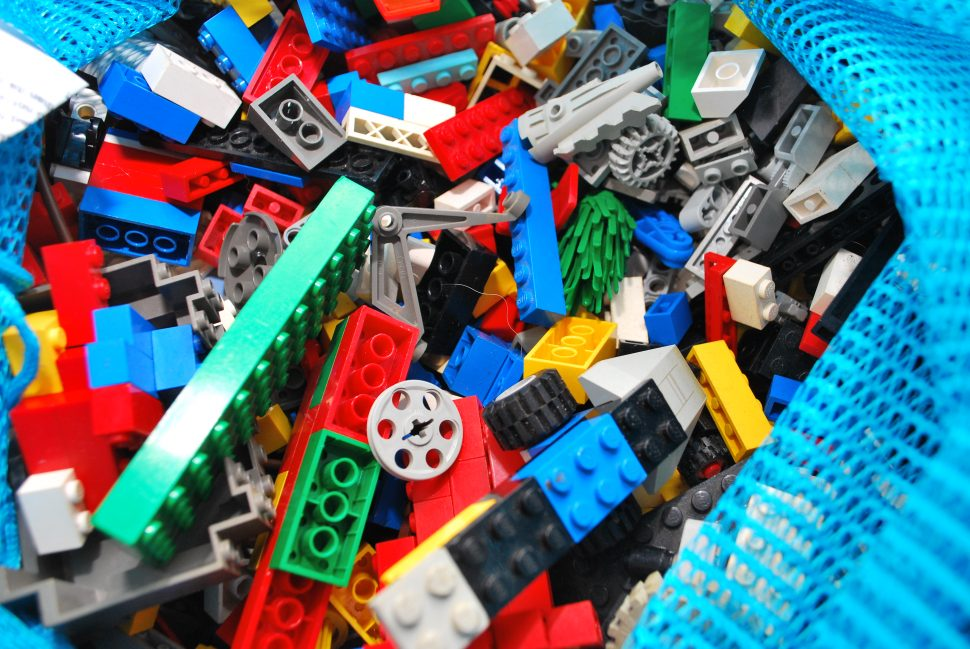
\includegraphics[height=0.45\textheight]{Images/Xilinx/FPGA/cool-wash-gettin-gallon-bag-legos-washing-lego-large-of-yellow-cheap-walmart-castle-bricks-little-small-ebay-big-giant-970x649}}

  \url{https://www.quora.com/What-is-FPGA-How-does-that-works }
\end{frame}


\begin{frame}{Xilinx 7nm Versal AI Core VC1902}
   \centerline{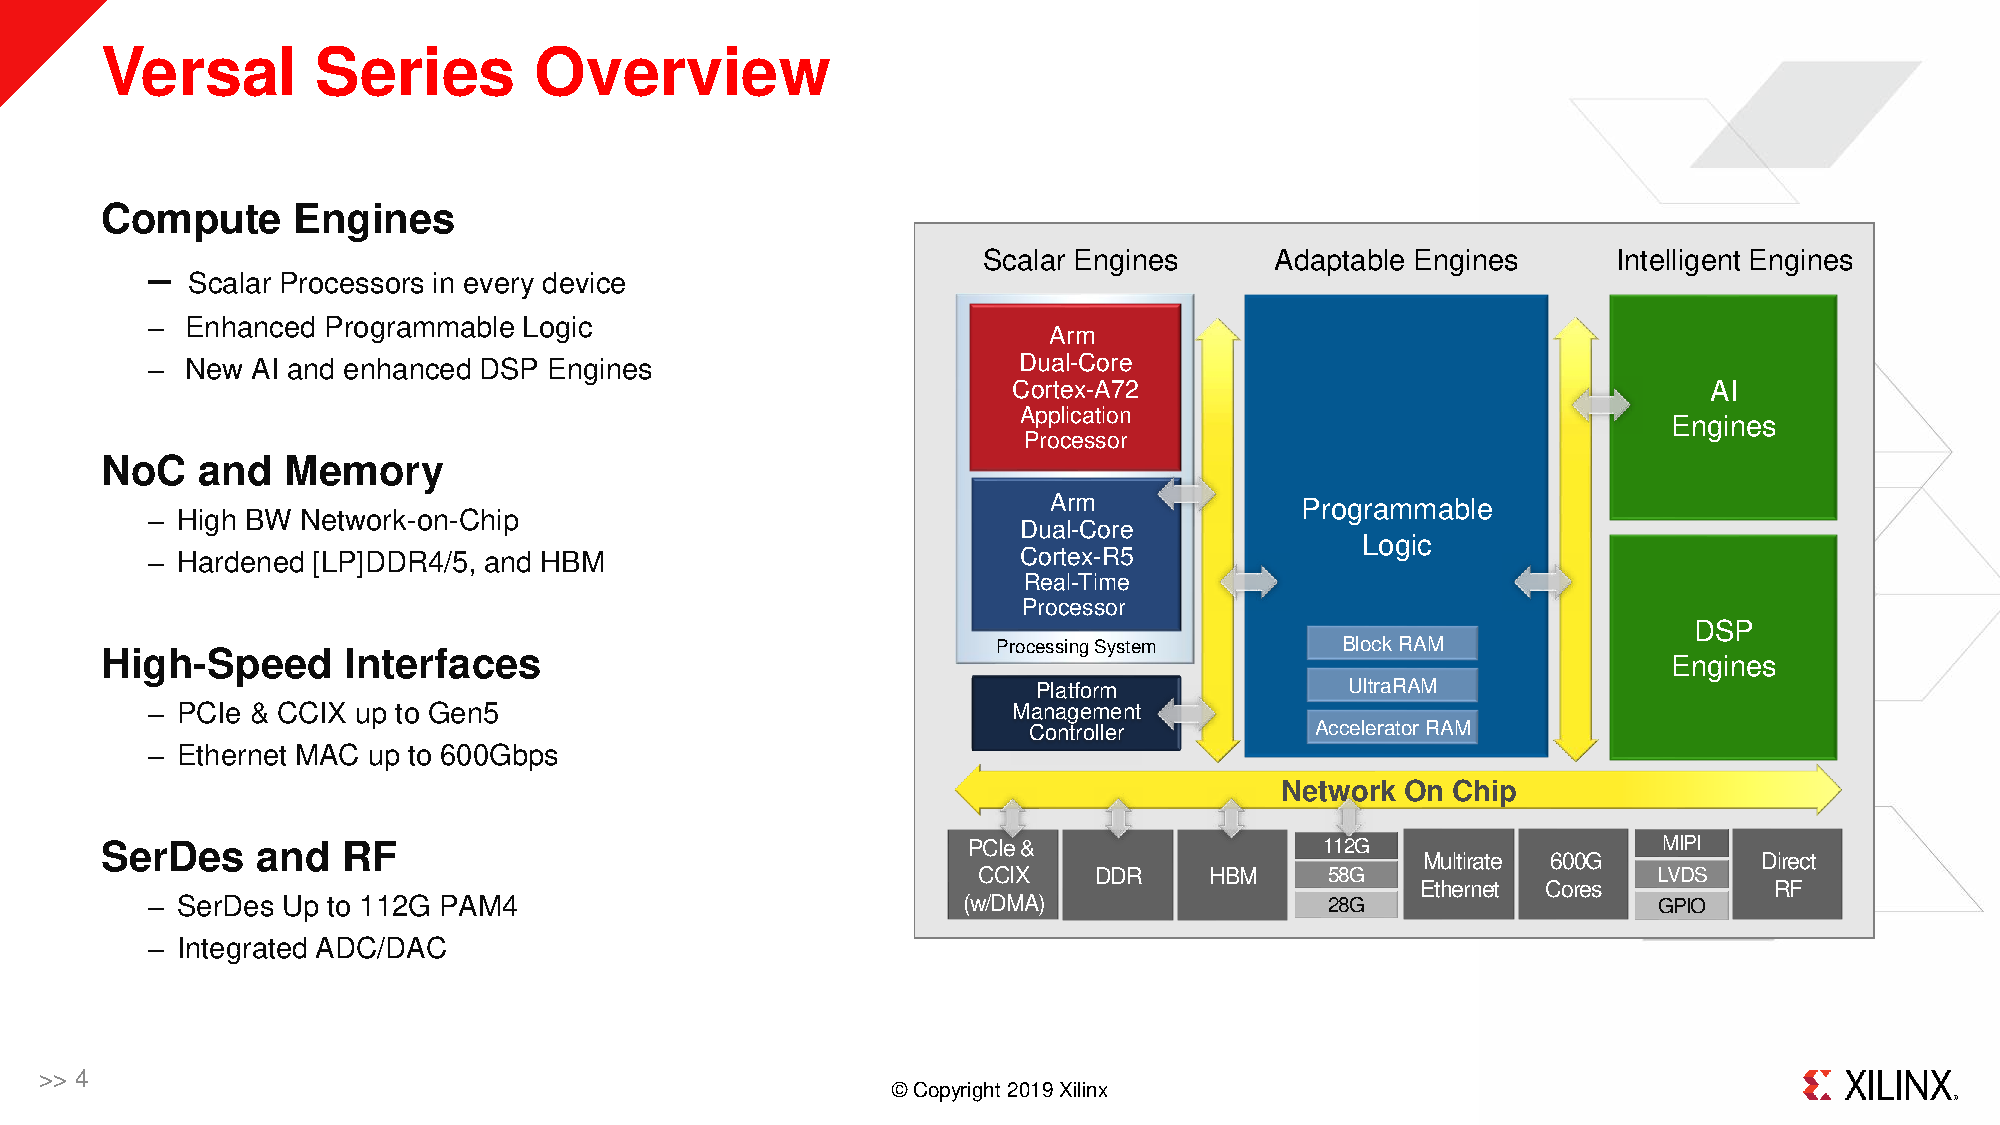
\includegraphics[height=0.95\vsize]{Xilinx/Versal/HotChips-2019/HC31_2_5_Xilinx_Versal_Hotchips31_Final_v2-slide4-Versal_serie_overview}}
\end{frame}

\begin{frame}{Not a completely new problem...}
  \begin{multicols}{2}
    \begin{itemize}
    \item SOLOMON
      \begin{itemize}
      \item Daniel L. Slotnick. � The SOLOMON computer. �
        \emph{Proceedings of the December 4-6, 1962, fall joint
          computer conference}. p.  97--107. \textcolor{red}{1962}
      \item Target application: \emph{``data reduction, communication,
          character recognition, optimization, guidance and control,
          orbit calculations, hydrodynamics, heat flow, diffusion,
          radar data processing, and numerical weather forecasting''}
      \item Diode + transistor logic in 10-pin TO5 package
      \end{itemize}
    \end{itemize}
    \centerline{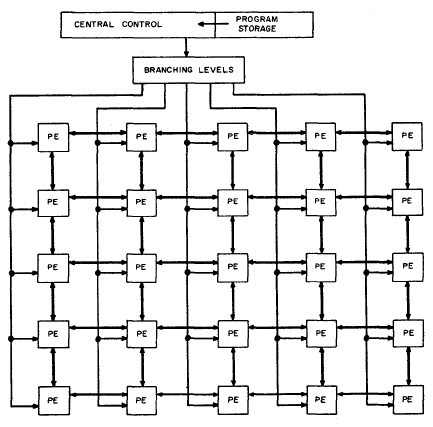
\includegraphics[width=0.9\hsize]{ordinateurs/SIMD/SOLOMON/p97-slotnick_PE_array_under_central_control}}
    But now not only for computing performance...
  \end{multicols}
\end{frame}


\begin{frame}{Stream computing: IBM 7950 Harvest 1962}
  \begin{multicols}{2}
    \begin{itemize}
    \item Coprocessor of the IBM Stretch (IBM 7030 Data Processing
      System)
      \begin{itemize}
      \item IBM 7951 Stream coprocessor ($3.10^6$ characters/s)
      \item IBM 7952 High performance core storage
      \item IBM 7955 Magnetic tape system, also known as TRACTOR
      \item IBM 7959 High speed I/O exchange
      \end{itemize}
    \item Installed NSA for cryptanalysis
    \end{itemize}
    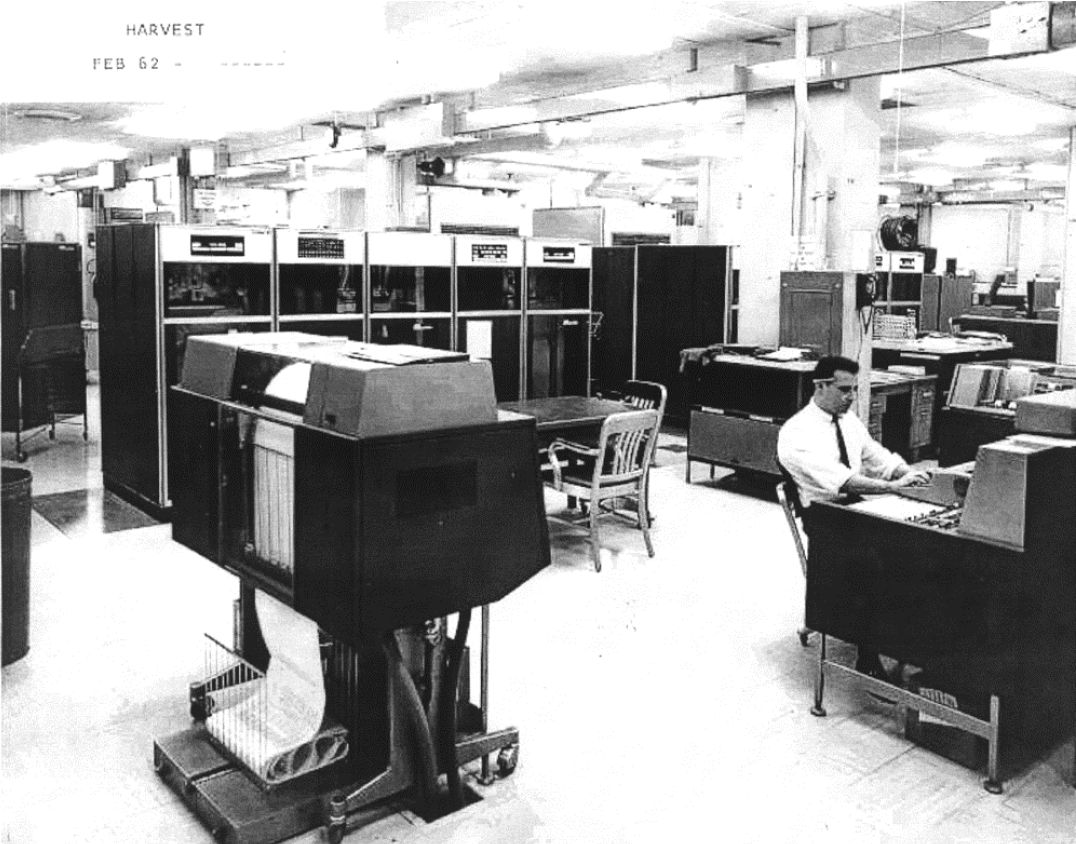
\includegraphics[width=\hsize]{ordinateurs/IBM/HARVEST}
  \end{multicols}
  \url{https://en.wikipedia.org/wiki/IBM_7950_Harvest}
\end{frame}


\begin{frame}{Typical modern MPSoC (for power consumption reasons)}
  What's new? Everything is on-chip now!!!
  \begin{itemize}
  \item Several \alert{CPU}
    \begin{itemize}
    \item Different kinds of CPU
    \end{itemize}
  \item Different kinds of \alert{accelerators}
    \begin{itemize}
    \item \alert{Vision}
    \item \alert{ML}
    \item \ldots
    \end{itemize}
  \item \alert{GPU}
  \item \alert{DSP}
  \item Some even with \alert{FPGA}
  \item Lot of I/O
  \item Different power domains
  \item Various on-chip memories
  \item \ldots
  \end{itemize}
\end{frame}


\section{Programming model}

\begin{frame}{All Programmable [with hardware mind set]}
  Programming style
  \begin{itemize}
  \item Anything resolves to writing 0 and 1 in (configuration) memory
    \begin{itemize}
    \item Great unification achieved !
    \item Well done !
    \item Problem solved !
    \end{itemize}
  \item Actually done by Eckert, Mauchly and Von Neumann around
    1944-1950\ldots{} \smiley
  \end{itemize}
\end{frame}


\begin{frame}{Huge programming dilemma: there's plenty of room at the top!}
  \centerline{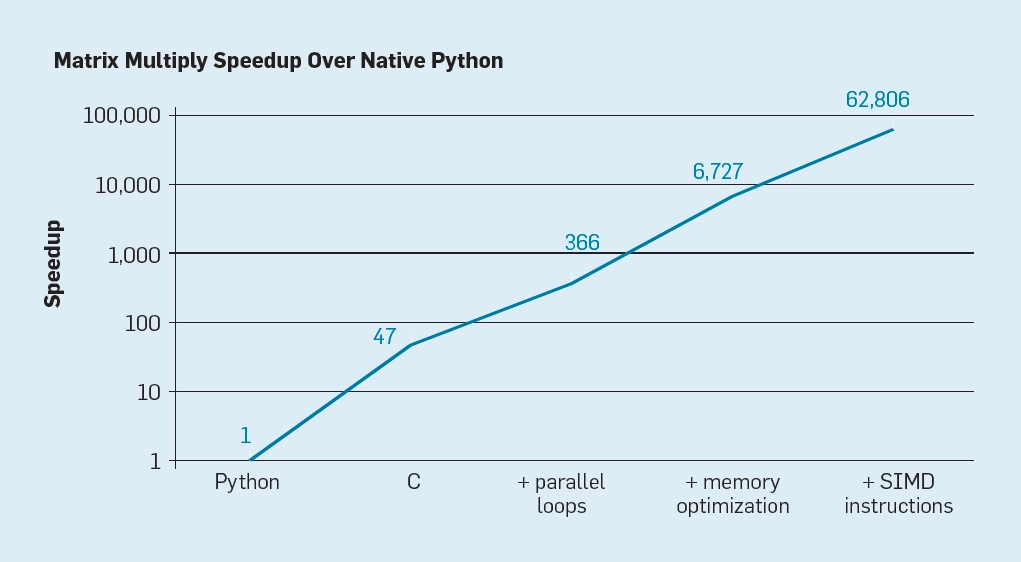
\includegraphics[height=0.85\vsize]{Languages/Python/Python_C_matrix_multiplication_performance}}
  \tiny
  Charles E. Leiserson, Neil C. Thompson, Joel S. Emer, Bradley
  C. Kuszmaul, Butler W. Lampson, Daniel Sanchez, and Tao B. Schardl,
  ``\emph{There's plenty of room at the top: What will drive growth in
    computer performance after Moore's Law ends?}'' unpublished
  manuscript submitted for publication, 2019.
\end{frame}


\begin{frame}{Heterogeneous computing
    [software \cancel{\alert{mind set}} nightmare]}
  \centerline{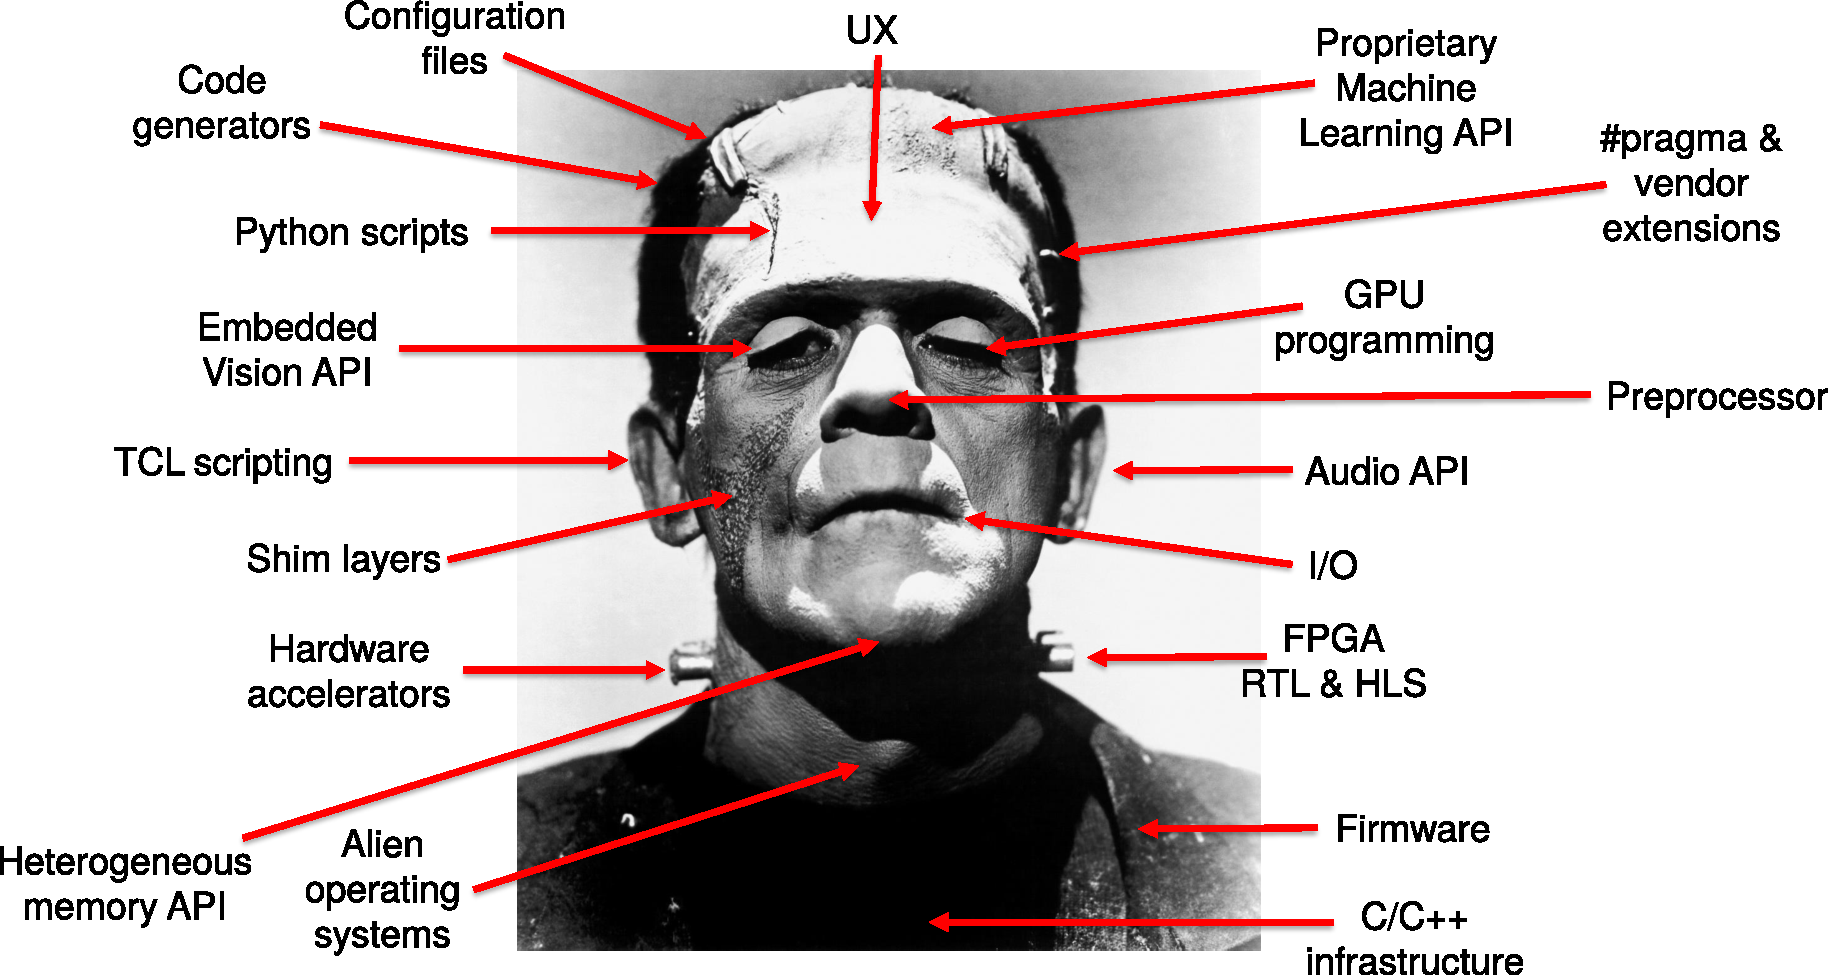
\includegraphics[height=0.9\vsize]
    {Images/Programming_Model/Frankenstein_programming_model}}
\end{frame}


\begin{frame}
  \centerline{\Huge � Can we do better ?}
\end{frame}


\section{Khronos Group: open standards for heterogeneous systems}

\SlideFromImageFile{Khronos/Members/Khronos-Member-Slide}

\SlideFromImageFile{Khronos/Members/About_Khronos_Slide-2018}


\subsection{OpenCL}

\begin{frame}{OpenCL}
  \centerline{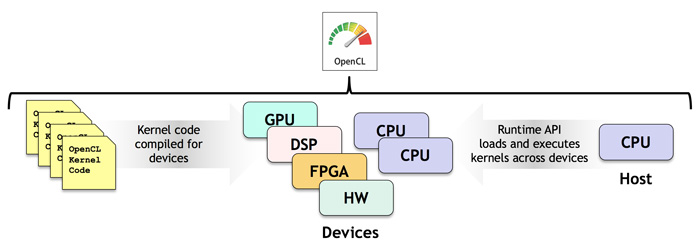
\includegraphics[width=\hsize]{Images/Languages/OpenCL/2015-api-opencl-1}}
  \begin{itemize}
  \item OpenCL: 2 host APIs and 2 kernel languages
    \begin{itemize}
    \item C Platform Layer API to query, select and initialize compute
      devices
    \item OpenCL C 2.0 and OpenCL C++ 2.2 kernel languages to write
      separate parallel code

    \item C Runtime API to build and execute kernels across multiple
      devices
    \end{itemize}
  \item One code tree can be executed on CPU, GPU, DSP, FPGA...
  \end{itemize}
\end{frame}


\begin{frame}{Architecture model: hierarchical organization}
  \centerline{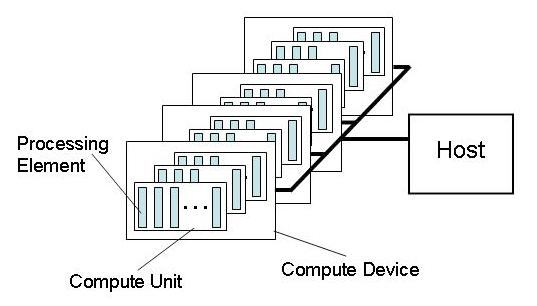
\includegraphics[width=0.7\textwidth]{Languages/OpenCL/OpenCL-2.0/compute-host-devices-model}}
  \begin{itemize}
  \item Host threads launch computational \emph{kernels} on
    \emph{accelerators}
  \end{itemize}
  \url{https://www.khronos.org/opencl}
\end{frame}


\begin{frame}{Execution model: embarrassingly parallel}
  \centerline{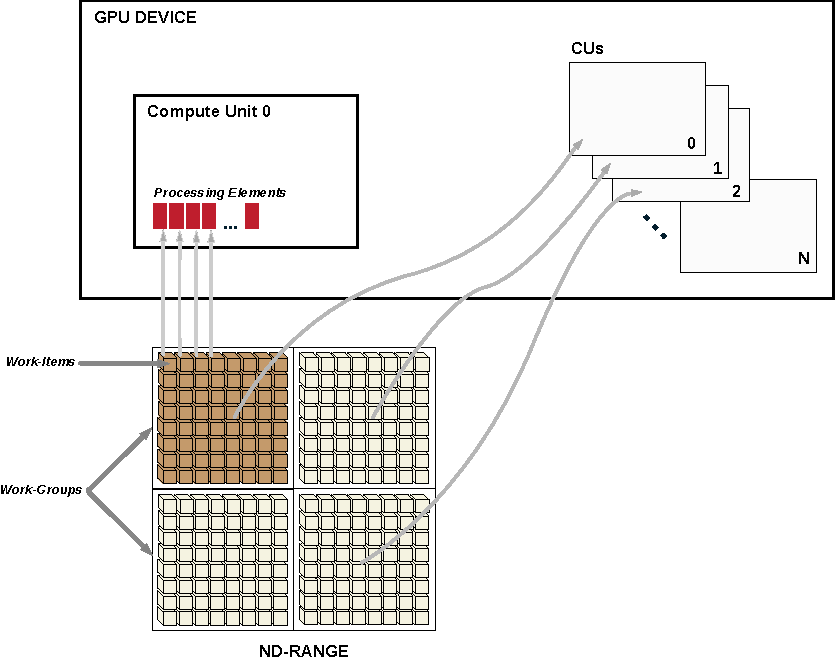
\includegraphics[height=0.9\textheight]{Languages/OpenCL/AMD_Accelerated_Parallel_Processing_OpenCL_Programming_Guide-rev-2.7/execution-model}}
\end{frame}


\begin{frame}{Memory model: express memory locality}
  \centerline{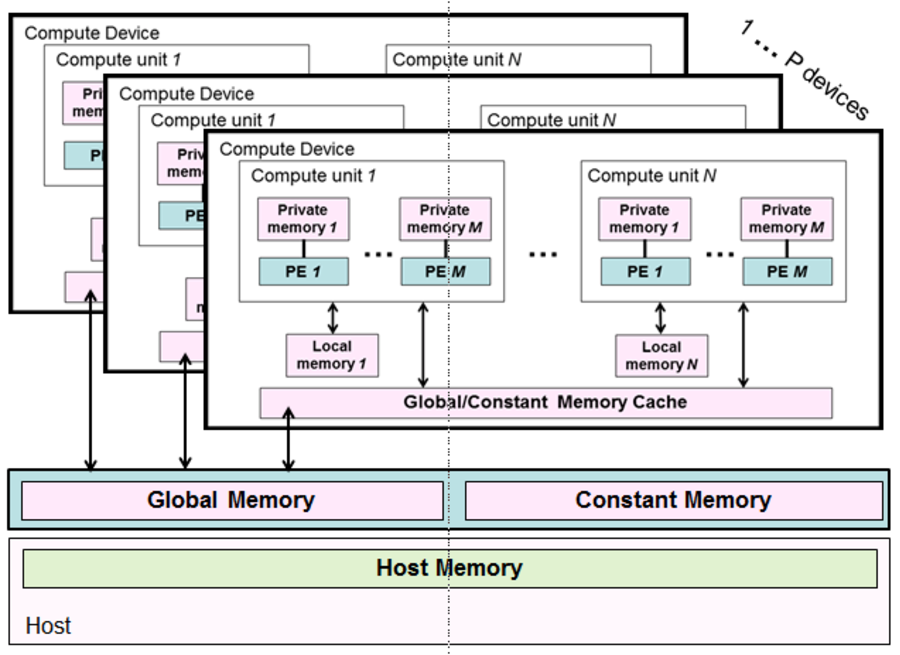
\includegraphics[height=0.9\textheight]{Languages/OpenCL/OpenCL-2.0/memory-model}}
\end{frame}


\subsection{SPIR-V}

\begin{frame}{Interoperability nightmare in heterogeneous computing \&
    graphics}
  \begin{itemize}
  \item $\exists$ Many programming languages for heterogeneous
    computing
    \begin{itemize}
    \item Writing compiler front-end may not be \emph{the} real
      value for a hardware vendor...
      \begin{itemize}
      \item Writing a C++ compiler from scratch is almost
        impossible...
      \end{itemize}
    \end{itemize}
  \item $\exists$ Many programming languages for writing shaders
  \item Convergence in computing (Compute Unit) \& graphics (Shader)
    architectures
    \begin{itemize}
    \item Same front-end \& middle-end compiler optimizations
    \end{itemize}
  \item Need for some non source-readable portable code for IP
    protection
  \end{itemize}
  \vavers Defining common low-level representation !
\end{frame}


\begin{frame}{Driving SPIR-V Open Source ecosystem}
    \centerline{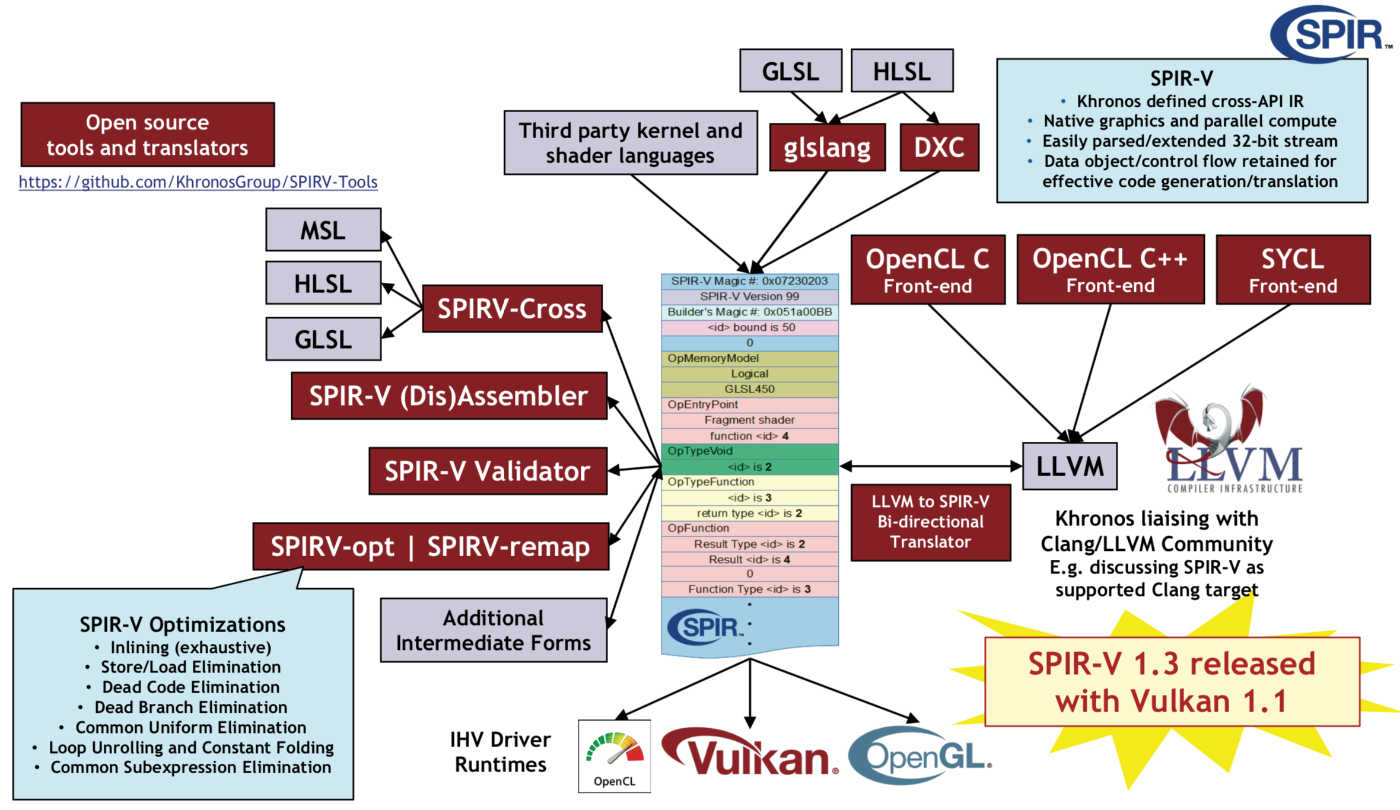
\includegraphics[width=0.95\hsize]{Images/Languages/SPIR-V/2018-spir-api-ecosystem}}
\end{frame}


\begin{frame}{OpenCL/OpenGL/Vulkan/SPIR(-V): the language way}
  \begin{itemize}
  \item Solve programming of heterogeneous accelerators
  \item Solve host-device interaction in a standard way
  \item Modeled according to graphics programming from the 90's \&
    GPU-focused
    \begin{itemize}
    \item Focused on portability across lot of GPU platforms
      % (the typical ``Eric Berdahl's (Adobe) use case'' \smiley)
      \begin{itemize}
      \item Fast JIT for platform adaptativity
      \end{itemize}
    \item What about the other 92\% architectures at HotChips 2019?
      \frownie
    \end{itemize}
  \item Not single-source \& single-language \frownie
    \begin{itemize}
    \item Part of the Frankenstein's programming model... \frownie
    \end{itemize}
  \item Require writing 2 unrelated programs using 2 different languages \frownie
    \begin{itemize}
    \item Host Device
    \end{itemize}
  \item Do not solve the global application problem \frownie
    \begin{itemize}
    \item No type-safety between host and device for generic code
    \item Unrelated memory address-spaces between host \& device code
    \item No global interprocedural \& cross host/device optimizations
      in compiler
    \end{itemize}
  \end{itemize}
\end{frame}


\section{SYCL}

\begin{frame}{Position argument}
  Which language for unified heterogeneous computing?
  \begin{itemize}
  \item \Attention Entry cost
  \item $\exists$ thousands of dead parallel languages...
    \begin{itemize}
    \item \Attention\Attention\Attention Exit cost
    \end{itemize}
  \item Use standard solutions with open source implementations
  \item Only the full application matter
  \item So a kernel language does not really matter
  \item Avoid stitching and Frankenstein programming
  \item Need an holistic approach
  \end{itemize}
\end{frame}


\subsection{C++}

\begin{frame}{Remember C++ ?}
  \begin{BoiteA}{2-line description by Bjarne Stroustrup}
    \begin{itemize}
    \item Direct mapping to hardware
    \item Zero-overhead abstraction
    \end{itemize}
  \end{BoiteA}
\end{frame}


\begin{frame}
  \centerline{\Huge � And what about post-modern C++ ?}
\end{frame}


\begin{frame}{ISO C++ committee proposal papers \& attendance}
  \centerline{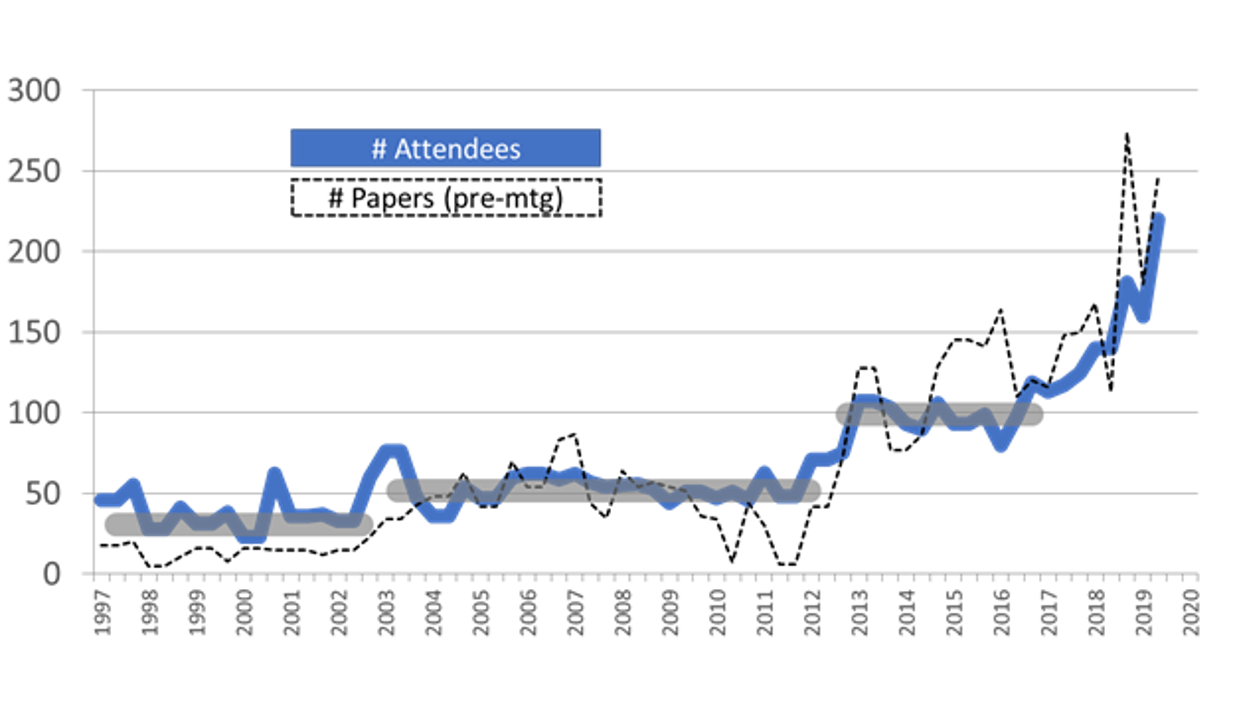
\includegraphics[height=\vsize]{Languages/C++/Meetings/2019-Cologne-attendance}}
\end{frame}


\begin{frame}[fragile]{Modern Python/Modern C++/Old C++}
  \begin{multicols}{2}
    \begin{itemize}
    \item Python 3.6
      \begin{lstlisting}
v = [ 1,2,3,5,7 ]
for e in v:
  print(e)
      \end{lstlisting}
    \item C++17
      \begin{lstlisting}
std::vector v { 1,2,3,5,7 };
for (auto e : v)
  std::cout << e << std::endl;
      \end{lstlisting}

      \columnbreak

    \item C++03
      \begin{lstlisting}
std::vector<int> v;
v.push_back(1);
v.push_back(2);
v.push_back(3);
v.push_back(5);
v.push_back(7);
for (std::vector<int>::iterator i =
       v.begin(); i != v.end(); ++i)
  std::cout << *i << std::endl;
      \end{lstlisting}
    \end{itemize}
  \end{multicols}
\end{frame}


\begin{frame}[fragile]{Back to Python... \uncover<2->{\\\vavers Modern C++ : like Python but with speed and type safety}}
  \begin{itemize}
  \item Python 3.x (interpreted):
    \begin{lstlisting}[language=Python]
def add(x, y): return x + y
print(add(2, 3))     # 5
print(add("2", "3")) # 23
print(add(2, "Boom")) # Fails at run-time :-(
    \end{lstlisting}
  \item<2-> Same in C++14 but {\color{red}compiled} + {\color{red}static
      compile-time type-checking}:
    \begin{lstlisting}
auto add = [] (auto x, auto y) { return x + y; };
std::cout << add(2, 3) << std::endl;       // 5
std::cout << add("2"s, "3"s) << std::endl; // 23
std::cout << add(2, "Boom"s) << std::endl; // ��� Does not compile !!! :-)
    \end{lstlisting}
    Without using templated code! \cancel{\texttt{template
        <typename>}} \smiley
  \end{itemize}
\end{frame}


\begin{frame}[fragile]{Generic variadic lambdas \& operator interpolation}
  \begin{lstlisting}
#include <iostream>
#include <string>
using namespace std::string_literals;
// Define an adder on anything.
// Use new C++14 generic variadic lambda syntax
auto add = [] (auto... args) {
  // Use new C++17 operator folding syntax (here from left)
  return (... + args);
};

int main() {
 std::cout << "The result is: " << add(1, 2, 3) << std::endl;
 std::cout << "The result is: " << add("begin"s, "end"s) << std::endl;
}
  \end{lstlisting}
  Without using templated code! \cancel{\texttt{template <typename>}}
  \smiley

  Try this example on
  \url{https://wandbox.org/permlink/LambcvLqmyaSV4JL}
\end{frame}


\begin{frame}{Make C++ more complex to make it\ldots simpler!}
  \begin{itemize}
  \item Modern C++ quite simpler to use
  \item But still compatible with old C++ \& C
    \begin{itemize}
    \item Globally more complex for\ldots implementers!
    \end{itemize}
  \item Keep \textbf{end-user only focused on simpler modern features}
  \item[\vavers] ISO C++ committee working on \textbf{C++ Core Guidelines}
    \begin{itemize}
    \item \url{http://isocpp.github.io/CppCoreGuidelines/CppCoreGuidelines}
    \end{itemize}
  \item Subliminal messages
    \begin{itemize}
    \item Learn modern C++\ldots and teach students or customers! \smiley
    \item Forget about what you know from old C/C++ \smiley
    \end{itemize}
  \end{itemize}
\end{frame}


\iffalse

\begin{frame}{1 C++ version/3 years \protect\vavers Parallelizing C++
    committee itself!}
  \begin{multicols}{2}
    \begin{itemize}
    \item Language rebooted in 2011
      \begin{itemize}
      \item[\vavers] Larger attraction \& interest
      \end{itemize}
    \item Is there any precedent of programming language developed
      cooperatively by of 200+ people democracy?
    \item[\vavers] Use... parallelism ! \smiley
      \begin{itemize}
      \item Generic working groups:
        \begin{itemize}
        \item Core Working Group. Library Working Group, Evolution
          Working Group, Library Evolution Working Group
        \end{itemize}
      \item Specialized Study Groups
        \begin{itemize}
        \item \alert{SG1, Concurrency:} Olivier Giroux
          (Nvidia). Concurrency, parallelism, SIMD, memory
          model... SYCL is a candidate here!
        \item \alert{SG6, Numerics:} Lawrence Crowl. Numerics topics,
          fixed point, decimal floating point, fractions, arbitrary
          precision...
        \item \alert{SG14, Game Development \& Low Latency:} Michael
          Wong (Codeplay): embedded systems, heterogeneous computing
        \end{itemize}
      \end{itemize}
    \item Production of Technical Specifications before
      standardization
      \begin{itemize}
      \item Implemented in several compilers
      \item Allow experiments in the fields
      \item Provide feedback to the ISO C++ Committee
      \end{itemize}
    \end{itemize}
  \end{multicols}
\end{frame}


\begin{frame}[fragile]{Position argument 2: start with modern C++...}
  \begin{itemize}
  \item Very successful \& ubiquitous language
    \begin{itemize}
    \item Millions of programmers
    \item Billions of users: any use of cars, IoT, IT, smartphone,
      Internet... depend on C/C++
    \end{itemize}
  \item Very active since C++11 (C++14, C++17, C++20...)
  \item Interoperability: seamless interaction with embedded world,
    libraries, OS, C...
  \item[\vavers] Unique existing position in embedded system to
    control the full stack!!!
  \item \alert{Full-stack}: combine both low-level aspects with
    high-level programming, multi-paradigm
    \begin{itemize}
    \item \alert{Pay only for what you need}
    \end{itemize}
  \item Open-source production-grade compilers (GCC \& Clang/LLVM) \&
    tools
    \begin{itemize}
    \item Implemented \alert{before} specification
      \begin{itemize}
      \item ... because it is too complex to do otherwise!!!
      \end{itemize}
    \end{itemize}
  \item Generic programming + classes can be used to define Domain
    Specific Embedded Language (DSEL)
  \item Not directly targeting heterogeneous computing...
    \begin{itemize}
    \item But extensible through classes (\vavers DSEL)
    \item Also extensible with \lstinline|#pragma| (already in Xilinx
      tools Vivado HLS, SDSoC \& SDAccel for FPGA) and attributes
    \end{itemize}
  \end{itemize}
\end{frame}


\fi

\subsection{SYCL as pure C++}

\begin{frame}[fragile]{Complete example of matrix addition in SYCL}
  \begin{multicols}{2}
    % triSYCL/tests/examples/simpler_parallel_matrix_add.cpp
    % Put it before to avoid overriding the listing
    \balloono{comment}{MatrixAdd}{24}{33}
    \balloon{comment}{MatrixAdd}{30}{32}
    \begin{lstlisting}[basicstyle=\scriptsize,name=MatrixAdd]
#include <CL/sycl.hpp>
#include <iostream>

using namespace cl::sycl;

constexpr size_t N = 2;
constexpr size_t M = 3;
using Matrix = float[N][M];

// Compute sum of matrices a and b into c
int main() {
 Matrix a = { { 1, 2, 3 }, { 4, 5, 6 } };
 Matrix b = { { 2, 3, 4 }, { 5, 6, 7 } };

 Matrix c;

 {// Create a queue to work on default device
  queue q;
  // Wrap some buffers around our data
  buffer A { &a[0][0], range { N, M } };
  buffer B { &b[0][0], range { N, M } };
  buffer C { &c[0][0], range { N, M } };
  // Enqueue some computation kernel task
  q.submit([&](handler& cgh) {
   // Define the data used/produced
   auto ka = A.get_access<access::mode::read>(cgh);
   auto kb = B.get_access<access::mode::read>(cgh);
   auto kc = C.get_access<access::mode::write>(cgh);
   // Create & call kernel named "mat_add"
   cgh.parallel_for<class mat_add>(range { N, M },
      [=](id<2> i) { kc[i] = ka[i] + kb[i]; }
   );
  }); // End of our commands for this queue
 } // End scope, so wait for the buffers to be released
 // Copy back the buffer data with RAII behaviour.
 std::cout << "c[0][2] = " << c[0][2] << std::endl;
 return 0;
}
    \end{lstlisting}
  \end{multicols}
\end{frame}


\begin{frame}{Asynchronous task graph model}
  \begin{itemize}
  \item Change example with initialization kernels instead of host?...
  \item Theoretical graph of an application described \emph{implicitly}
    with kernel tasks using buffers through accessors

    \medskip

    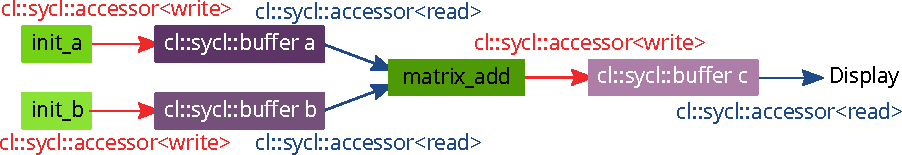
\includegraphics[width=\hsize]{Pictures/unscheduled_task_graph}

  \item Possible schedule by SYCL runtime:

    \centerline{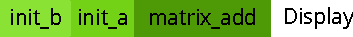
\includegraphics[width=0.4\hsize]{Pictures/scheduled_task_graph}}

    \item[\vavers] Automatic overlap of kernels \& communications
      \begin{itemize}
      \item Even better when looping around in an application
      \item Assume it will be translated into pure back-end event graph
      \item Runtime uses as many threads \& back-end queues as necessary
      \end{itemize}
  \end{itemize}
\end{frame}


\begin{frame}[fragile]{Task graph programming --- the full code}
  \vspace{-.75cm}
  \begin{multicols}{2}
    % Put it before to avoid overriding the listing
    \balloono{comment}{TaskGraph}{18}{27}
    \balloon{comment}{TaskGraph}{23}{26}
    % Adjust for the column break, because it is not compatible with
    \balloono{comment}{TaskGraph}{30}{35}
    % Repeat after the column break
    \balloono{comment}{TaskGraph}{40}{45}
    % Adjust for the column break, because it is not compatible with
    \balloon{comment}{TaskGraph}{41}{44}
    \balloono{comment}{TaskGraph}{47}{60}
    \balloon{comment}{TaskGraph}{56}{59}
    \begin{tikzpicture}[remember picture,overlay]
      \draw [overlay,->,very thick,red] (pic cs:PA) to[bend left] (pic cs:CA);
      \draw [overlay,->,very thick,red] (pic cs:PB) to[bend left] (pic cs:CB);
      \draw [overlay,->,very thick,red] (pic cs:PC) to[bend right] (pic cs:CC);
    \end{tikzpicture}
    % triSYCL/tests/examples/demo_parallel_matrices_add.cpp
    \begin{lstlisting}[basicstyle=\tiny,name=TaskGraph]
#include <CL/sycl.hpp>
#include <iostream>
using namespace cl::sycl;
// Size of the matrices
constexpr size_t N = 2000;
constexpr size_t M = 3000;
int main() {
  { // By sticking all the SYCL work in a {} block, we ensure
    // all SYCL tasks must complete before exiting the block.
    // Create a queue to work on default device
    queue q;
    // Create some 2D buffers of float for our matrices
    buffer<double, 2> a({ N, M });
    buffer<double, 2> b({ N, M });
    buffer<double, 2> c({ N, M });

    // Launch a first asynchronous kernel to initialize a
    q.submit([&](auto &cgh) {
        // The kernel write a, so get a write accessor on it
        auto A = a.get_access<access::mode::write>(cgh);�\tikzmark{PA}�

        // Enqueue parallel kernel on a N*M 2D iteration space
        cgh.parallel_for<class init_a>({ N, M },
                           [=] (auto index) {
                             A[index] = index[0]*2 + index[1];
                           });
      });

    // Launch an asynchronous kernel to initialize b
    q.submit([&](auto &cgh) {
        // The kernel write b, so get a write accessor on it
        auto B = b.get_access<access::mode::write>(cgh);�\tikzmark{PB}�
        /* From the access pattern above, the SYCL runtime detect
           this command_group is independant from the first one
           and can be scheduled independently */




        // Enqueue a parallel kernel on a N*M 2D iteration space
        cgh.parallel_for<class init_b>({ N, M },
                           [=] (auto index) {
                             B[index] = index[0]*2014 + index[1]*42;
                           });
      });
    // Launch an asynchronous kernel to compute matrix addition c = a + b
    q.submit([&](auto &cgh) {
        // In the kernel a and b are read, but c is written
        auto A = �\tikzmark{CA}�a.get_access<access::mode::read>(cgh);
        auto B = �\tikzmark{CB}�b.get_access<access::mode::read>(cgh);
        auto C = �\tikzmark{PC}�c.get_access<access::mode::write>(cgh);
        // From these accessors, the SYCL runtime will ensure that when
        // this kernel is run, the kernels computing a and b completed

        // Enqueue a parallel kernel on a N*M 2D iteration space
        cgh.parallel_for<class matrix_add>({ N, M },
                                       [=] (auto index) {
                                         C[index] = A[index] + B[index];
                                       });
      });
    /* Request an access to read c from the host-side. The SYCL runtime
       ensures that c is ready when the accessor is returned */
    auto C = �\tikzmark{CC}�c.get_access<access::mode::read, access::target::host_buffer>();
    std::cout << std::endl << "Result:" << std::endl;
    for(size_t i = 0; i < N; i++)
      for(size_t j = 0; j < M; j++)
        // Compare the result to the analytic value
        if (C[i][j] != i*(2 + 2014) + j*(1 + 42)) {
          std::cout << "Wrong value " << C[i][j] << " on element "
                    << i << ' ' << j << std::endl;
          exit(-1);
        }
  }
  std::cout << "Good computation!" << std::endl;
  return 0;
}
    \end{lstlisting}
  \end{multicols}
\end{frame}



\begin{frame}{SYCL = Pure C++ based DSEL}
  \setbeamertemplate{itemize/enumerate body begin}{\scriptsize}
  \setbeamertemplate{itemize/enumerate subbody begin}{\scriptsize}
  Implement concepts useful for \alert{heterogeneous computing}
  % vspace{-1cm}
  \begin{multicols}{2}
    \begin{itemize}
    \item \alert{Modern C++ features available for accelerators}
      \begin{itemize}
      \item Builds on the features of C++11, with additional support
        for more modern C++
      \item Enables ISO C++17 Parallel STL programs to be accelerated
      \item Simplifies the porting of existing templated C++ Libraries
        and frameworks, i.e., Eigen, TensorFlow\ldots
      \end{itemize}
    \item Generic heterogeneous computing model
      \begin{itemize}
      \item On CPUs, GPUs, FPGAs\ldots
      \item Hierarchical parallelism
      \end{itemize}
    \item Portability across platforms and compilers
    \item \alert{Single source programming model}
      \begin{itemize}
      \item Better type safety
      \item Simpler and cleaner code
      \item Compiled host and device code
      \end{itemize}
    \item \alert{Asynchronous task graph}
      \begin{itemize}
      \item Describes implicitly with kernel tasks using
        \alert{buffers} through \alert{accessors}
      \item Automatic overlap kernel executions and communications
      \end{itemize}
    \item \alert{Only Queues needed to direct computations on devices}
      \begin{itemize}
      \item Runtime handles multiple platforms, devices, and context
      \end{itemize}
    \item \alert{Interoperability} with multiple languages according
      to back-end
      \begin{itemize}
      \item OpenCL, OpenGL, Vulkan, OpenVX, DirectX, CUDA...
      \end{itemize}
    \item \alert{Host fall-back}
      \begin{itemize}
      \item Easily develops and debugs applications on the host
        without a device
      \item No specific compiler needed for experimenting on host
      \item \alert{Full system architectural emulation for free!}
      \end{itemize}
    \end{itemize}
  \end{multicols}
\end{frame}


\begin{frame}{Remember the OpenCL execution model?}
  \centerline{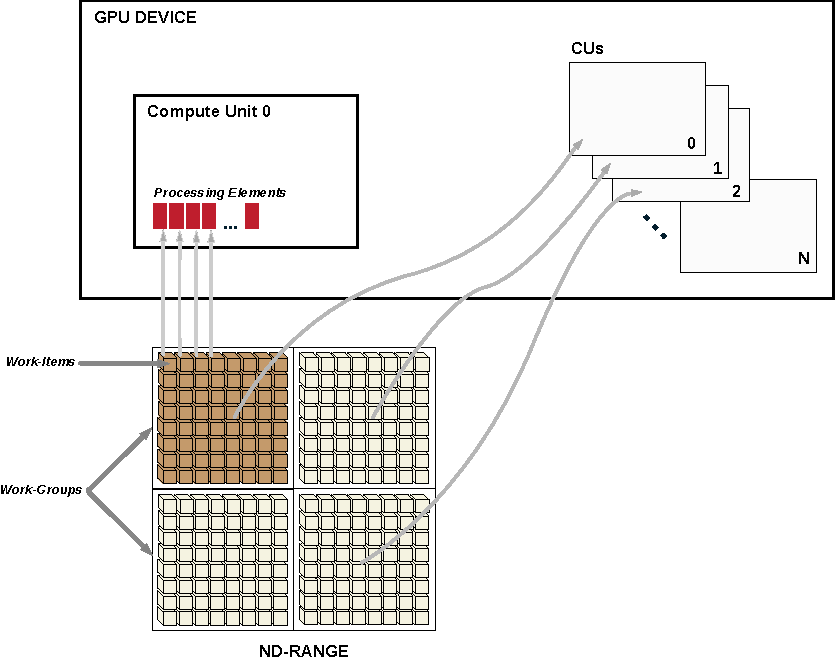
\includegraphics[height=0.7\textheight]{Languages/OpenCL/AMD_Accelerated_Parallel_Processing_OpenCL_Programming_Guide-rev-2.7/execution-model}}
  How to control this 2-level parallelism in a a simple way?
\end{frame}


\begin{frame}[fragile]{From work-groups \& work-items to hierarchical
    parallelism}
  \begin{multicols}{2}
    \balloon{comment}{HierarchicalParallelism}{18}{21}
    \balloon{comment}{HierarchicalParallelism}{32}{40}
    \balloon{comment}{HierarchicalParallelism}{44}{51}
    \balloon{comment}{HierarchicalParallelism}{54}{56}
    \begin{lstlisting}[basicstyle=\tiny,name=HierarchicalParallelism]
// Launch a 1D convolution filter
my_queue.submit([&](handler &cgh) {
  auto in_access = inputB.get_access<access::mode::read>(cgh);
  auto filter_access = filterB.get_access<access::mode::read>(cgh);
  auto out_access = outputB.get_access<access::mode::write>(cgh);

  // Iterate on all the work-group
  cgh.parallel_for_work_group<class convolution>({ size,
                                                   groupsize },
    [=](group<> group) {
      �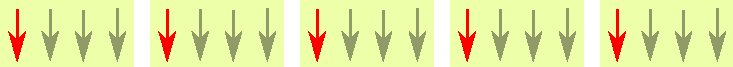
\includegraphics[height=2em]{Images/Languages/OpenMP/teams}�
      // These are OpenCL local variables used as a cache
      float filterLocal[2*radius + 1];
      float localData[blocksize + 2*radius];
      float convolutionResult[blocksize];
      range<1> filterRange { 2*radius + 1 };
      // Iterate on filterRange work-items
      group.parallel_for_work_item(filterRange, [&](h_item<1> tile) {
        �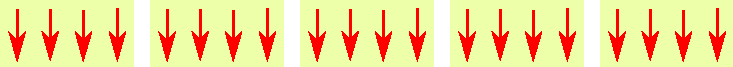
\includegraphics[height=2em]{Images/Languages/OpenMP/parallel_distribute}�
        filterLocal[tile] = filter_access[tile];
      });
      // There is an implicit work-group barrier here

      range<1> inputRange{ blocksize + 2*radius };






      // Iterate on inputRange work-items
      group.parallel_for_work_item(inputRange, [&](h_item<1> tile) {
        �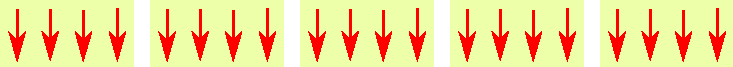
\includegraphics[height=2em]{Images/Languages/OpenMP/parallel_distribute}�
        float val = 0.f;
        int readAddress = tile.get_global_id() - radius;
        if (readAddress >= 0 && readAddress < size)
          val = in_access[readAddress];

        localData[tile] = val;
      });
      // There is an implicit work-group barrier here

      // Iterate on all the work-items
      group.parallel_for_work_item([&](h_item<1> tile) {
        �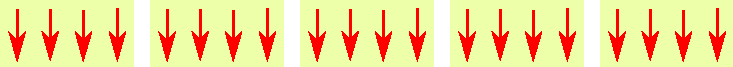
\includegraphics[height=2em]{Images/Languages/OpenMP/parallel_distribute}�
        float sum = 0.f;
        for (unsigned offset = 0; offset < radius; ++offset)
          sum += filterLocal[offset]*localData[tile + offset + radius];
        float result = sum/(2*radius + 1);
        convolutionResult[tile] = result;
      });
      // There is an implicit work-group barrier here
      // Iterate on all the work-items
      group.parallel_for_work_item(group, [&](h_item<1> tile)
        out_access[tile.get_global_id(0)] = convolutionResult[tile];
      });
      // There is an implicit work-group barrier here
    });
  });
    \end{lstlisting}
  \end{multicols}
\end{frame}


\begin{frame}[fragile]{Very close to OpenMP 5 style! \smiley}
  \begin{itemize}
  \item Easy to understand the concept of work-groups
  \item Easy to write work-group only code
    \begin{itemize}
    \item Local variables inside \lstinline|parallel_for_work_group|
      are mapped to OpenCL \lstinline|local| or CUDA
      \lstinline|shared| address space
    \end{itemize}
  \item Replace code + barriers with several
    \lstinline|parallel_for_work_item()|
    \begin{itemize}
    \item Performance-portable between CPU and device
    \item No need to think about barriers (automatically deduced)
    \item Easier to compose components \& algorithms
    \item Ready for future device with non uniform work-group size
    \end{itemize}
  \end{itemize}
\end{frame}


\begin{frame}{OpenCL interoperability mode}
  \begin{itemize}
  \item SYCL $\equiv$ very generic parallel model
  \item Specific to SYCL: OpenCL interoperability if implementation
    based on OpenCL
  \item Can interact with OpenCL/Vulkan/OpenGL/... program or
    libraries \emph{with no} overhead
  \item Value for OpenCL programmers: keep high-level features of SYCL
    \begin{itemize}
    \item Simplify boilerplate and housekeeping
      \begin{itemize}
      \item No explicit buffer transfer
      \item Task and data dependency graphs
      \item Templated C++ code
      \end{itemize}
    \end{itemize}
  \item The user can call any existing OpenCL kernel
    \begin{itemize}
    \item Even HLS C++ \& RTL FPGA kernels !
    \item Avoid writing painful OpenCL C/C++ host code
    \end{itemize}
  \end{itemize}
\end{frame}


\begin{frame}[fragile]{Example of SYCL program running explicit OpenCL code}
  \begin{multicols}{2}
    % Put it before to avoid overriding the listing
    \balloon{comment}{OpenCLInterop}{37}{41}
    \balloono{comment}{OpenCLInterop}{51}{58}
    \balloon{comment}{OpenCLInterop}{57}{57}
    % triSYCL/tests/examples/simpler_parallel_matrix_add.cpp
    \begin{lstlisting}[basicstyle=\tiny,name=OpenCLInterop]
#include <iostream>
#include <iterator>
#include <boost/compute.hpp>
#include <boost/test/minimal.hpp>

#include <CL/sycl.hpp>

using namespace cl::sycl;

constexpr size_t N = 3;
using Vector = float[N];

int test_main(int argc, char *argv[]) {
  Vector a = { 1, 2, 3 };
  Vector b = { 5, 6, 8 };
  Vector c;

  // Construct the queue from the defaul OpenCL one
  queue q { boost::compute::system::default_queue() };

  // Create buffers from a & b vectors
  buffer<float> A { std::begin(a), std::end(a) };
  buffer<float> B { std::begin(b), std::end(b) };

  {
    // A buffer of N float using the storage of c
    buffer<float> C { c, N };







    // Construct an OpenCL program from the source string
    auto program = boost::compute::program::create_with_source(R"(
      __kernel void vector_add(const __global float *a,
                               const __global float *b,
                               __global float *c) {
        c[get_global_id(0)] = a[get_global_id(0)] + b[get_global_id(0)];
      }
      )", boost::compute::system::default_context());

    // Build a kernel from the OpenCL kernel
    program.build();

    // Get the OpenCL kernel
    kernel k { boost::compute::kernel { program, "vector_add" } };

    // Launch the vector parallel addition
    q.submit([&](handler &cgh) {
        /* The host-device copies are managed transparently by these
           accessors: */
        cgh.set_args(A.get_access<access::mode::read>(cgh),
                     B.get_access<access::mode::read>(cgh),
                     C.get_access<access::mode::write>(cgh));
        cgh.parallel_for(N, k);
      }); //< End of our commands for this queue
  } //< Buffer C goes out of scope and copies back values to c

  std::cout << std::endl << "Result:" << std::endl;
  for (auto e : c)
    std::cout << e << " ";
  std::cout << std::endl;

  return 0;
}
    \end{lstlisting}
  \end{multicols}
\end{frame}


\begin{frame}[fragile]{C++17 STL has parallel algorithms now}
  \begin{itemize}
  \item Parallel STL now in C++17
    \url{https://en.cppreference.com/w/cpp/algorithm/sort}
\begin{lstlisting}
// Current C++11: standard sequential sort
std::sort(vec.begin(), vec.end());
// C++17: permitting parallel execution and vectorization as well
sort(std::execution::par_vec, vec.begin(), vec.end());
\end{lstlisting}
  \item Easy to implement in SYCL
    \begin{itemize}
    \item Could even be extended to give a kernel name (profile,
      debug...):
    \item Load balancing between CPU and accelerator
    \end{itemize}
\begin{lstlisting}
sycl_policy<class kernelName1> pol;
sort(pol, begin(vec), end(vec));

sycl_policy<class kernelName2> pol2;
// But SYCL allows OpenCL intrinsics in the operation too
for_each(pol2, vec.begin(), vec.end(),
         [](float & ans) { ans += cl::sycl::sin(ans); });
\end{lstlisting}
  \end{itemize}
  Open Source implementation \smiley{}
  \url{https://github.com/KhronosGroup/SyclParallelSTL}
\end{frame}


\subsection{The power of single source}

\begin{frame}{Single-source C++ enables generic libraries}
  �How to create a generic vector adder taking any number of vectors
  of any type?

  Not possible to do this with OpenCL C or OpenCL C++\ldots Not
  single-source C++ ! \frownie
  \begin{itemize}
  \item Single-source is the strength of CUDA!
    \begin{itemize}
    \item Allow generic programming for heterogeneous computing
      on... Nvidia GPU
    \item Type safety across host/device boundary
    \item Avoid spaghetti Frankenstein's programming of
      OpenCL/OpenGL/Vulkan
    \item Based on widely used multi-paradigm C++ language
    \item But not cross-platform, not multi-vendor, no DSP, no FPGA or
      other accelerators... \frownie
    \end{itemize}
  \item[\vavers] SYCL: portable cross-vendor single-source C++
    standard from Khronos
  \item This explains why TensorFlow/Eigen uses CUDA or SYCL with
    C++\ldots
\end{itemize}
\end{frame}


\begin{frame}[fragile]{Generic adder in 25 lines of SYCL \& C++17}
  \begin{multicols}{2}
    \begin{lstlisting}[basicstyle=\tiny]
auto generic_adder = [] (auto... inputs) {
  // Use a tupple of heterogeneous buffers to wrap the inputs
  auto a = boost::hana::make_tuple(
    buffer<typename decltype(inputs)::value_type>
      { std::begin(inputs), std::end(inputs) }...);
  // The basic computation
  auto compute = [] (auto args) {
    // f(... f(f(f(x1, x2), x3), x4) ..., xn)
    return boost::hana::fold_left(args, [] (auto a, auto b)
                                           { return a + b; });
  };
  // Use the range of the first argument as the range
  // of the result and computation
  auto size = a[0_c].get_count();
  // Infer the type of the output from 1 computation on inputs
  using return_value_type = decltype
    (compute(boost::hana::make_tuple(*std::begin(inputs)...)));
  // Allocate the buffer for the result
  buffer<return_value_type> output { size };
  // Submit a command-group to the device
  queue {}.submit([&] (handler& cgh) {
      // Define the data used as a tuple of read accessors
      auto ka = boost::hana::transform(a, [&] (auto b) {
          return b.template get_access<access::mode::read>(cgh);
        });
      // Data are produced to a write accessor to the output buffer
      auto ko = output.template
        get_access<access::mode::discard_write>(cgh);

      // Define the data-parallel kernel
      cgh.parallel_for<class gen_add>(size, [=] (id<1> i) {
          // Pack operands an elemental computation in a tuple
          auto operands =
            boost::hana::transform(ka, [&] (auto acc) {
              return acc[i];
            });
          // Assign computation on the operands to the elemental result
          ko[i] = compute(operands);
        });
  });
  // Return a host accessor on the output buffer
  return output.template get_access<access::mode::read_write>();
};


int main() {
  std::vector<int> u { 1, 2, 3 };
  std::vector<float> v { 5, 6, 7 };
  for (auto e : generic_adder(u, v))
    std::cout << e << ' ';
  std::cout << std::endl;
  std::vector<double> a { 1, 2.5, 3.25, 10.125 };
  std::set<char> b { 5, 6, 7, 2 };
  std::list<float> c { -55, 6.5, -7.5, 0 };
  for (auto e : generic_adder(a, b, c))
    std::cout << e << ' ';
  std::cout << std::endl;
  return 0;
}
    \end{lstlisting}
    \alert{6 8 10}

    \alert{52 14 1.75 17.125}
  \end{multicols}
\end{frame}


\begin{frame}[fragile]{Generic \alert{executor} in 25 lines of SYCL \& C++17}
  \begin{multicols}{2}
    \begin{lstlisting}[basicstyle=\tiny]
auto generic_executor = [] (auto op, auto... inputs) {
  // Use a tupple of heterogeneous buffers to wrap the inputs
  auto a = boost::hana::make_tuple(
    buffer<typename decltype(inputs)::value_type>
      { std::begin(inputs), std::end(inputs) }...);
  // The element-wise computation
  auto compute = [] (auto args) {
    // f(... f(f(f(x1, x2), x3), x4) ..., xn)
    return boost::hana::fold_left(args, op);
  };
  // Use the range of the first argument as the range
  // of the result and computation */
  auto size = a[0_c].get_count();
  // Infer the type of the output from 1 computation on inputs
  using return_value_type = decltype
    (compute(boost::hana::make_tuple(*std::begin(inputs)...)));
  // Allocate the buffer for the result
  buffer<return_value_type> output { size };
  // Submit a command-group to the device
  queue {}.submit([&] (handler& cgh) {
      // Define the data used as a tuple of read accessors
      auto ka = boost::hana::transform(a, [&] (auto b) {
          return b.template get_access<access::mode::read>(cgh);
        });
     // Data are produced to a write accessor to the output buffer
      auto ko = output.template
        get_access<access::mode::discard_write>(cgh);
      // Define the data-parallel kernel
      cgh.parallel_for<class gen_add>(size, [=] (id<1> i) {
          // Pack operands an elemental computation in a tuple
          auto operands =
            boost::hana::transform(ka, [&] (auto acc) {
              return acc[i];
            });
          // Assign computation on the operands to the elemental result
          ko[i] = compute(operands);
        });
  });
  // Return a host accessor on the output buffer
  return output.template get_access<access::mode::read_write>();
};


int main() {
  std::vector<int> u { 1, 2, 3 };
  std::vector<float> v { 5, 6, 7 };
  for (auto e : generic_executor([] (auto x, auto y)
                                    { return x + y; }, u, v))

    std::cout << e << ' ';
  std::cout << std::endl;
  std::vector<double> a { 1, 2.5, 3.25, 10.125 };
  std::set<char> b { 5, 6, 7, 2 };
  std::list<float> c { -55, 6.5, -7.5, 0 };
  for (auto e : generic_executor([] (auto x, auto y)
                                    { return 3*x - 7*y; },
    std::cout << e << ' ';
  std::cout << std::endl;
  return 0;
}
    \end{lstlisting}
    \alert{6 8 10}

    \alert{ 352 -128 -44.25 -55.875}
  \end{multicols}
\end{frame}


\begin{frame}[fragile]{Modern metaprogramming as\ldots hardware design tool}
  \begin{itemize}
  \item Alternative implementation of
    \begin{lstlisting}[basicstyle=\small]
auto compute = [] (auto args) {
  return boost::hana::fold_left(args, [] (auto a, auto b) { return a + b; });
}; // f(... f(f(f(x1, x2), x3), x4) ..., xn)
    \end{lstlisting}
    \begin{itemize}
    \item Possible to use other Boost.Hana algorithms to add some
      hierarchy in the computation (Wallace's tree...)
    \item Or to sort by type to minimize the hardware usage starting
      with ``smallest'' types
    \end{itemize}
  \item Metaprogramming allows various implementations according to
    the types, sizes\ldots
    \begin{itemize}
    \item Kernel fusion, pipelined execution\ldots
    \item Codeplay VisionCpp, Eigen kernel fusion, Halide DSL\ldots
    \item In sync with C++ proposal on executors \& execution contexts
    \end{itemize}
  \item Introspection \& metaclasses will allow quite more!
    \begin{itemize}
    \item Generative programming\ldots
      h\url{ttp://www.open-std.org/jtc1/sc22/wg21/docs/papers/2017/p0707r2.pdf}
      \begin{itemize}
      \item Mind-blowing\ldots
        \url{https://www.youtube.com/watch?v=4AfRAVcThyA}
      \end{itemize}
    \item Express directly and specialize code for each PE of a CGRA
      for example
    \end{itemize}
  \item Imagine if SystemC was invented with this future C++ instead
    of C++98\ldots
  \end{itemize}
\end{frame}


\section{Implementations}

\begin{frame}{Known implementations of SYCL}
  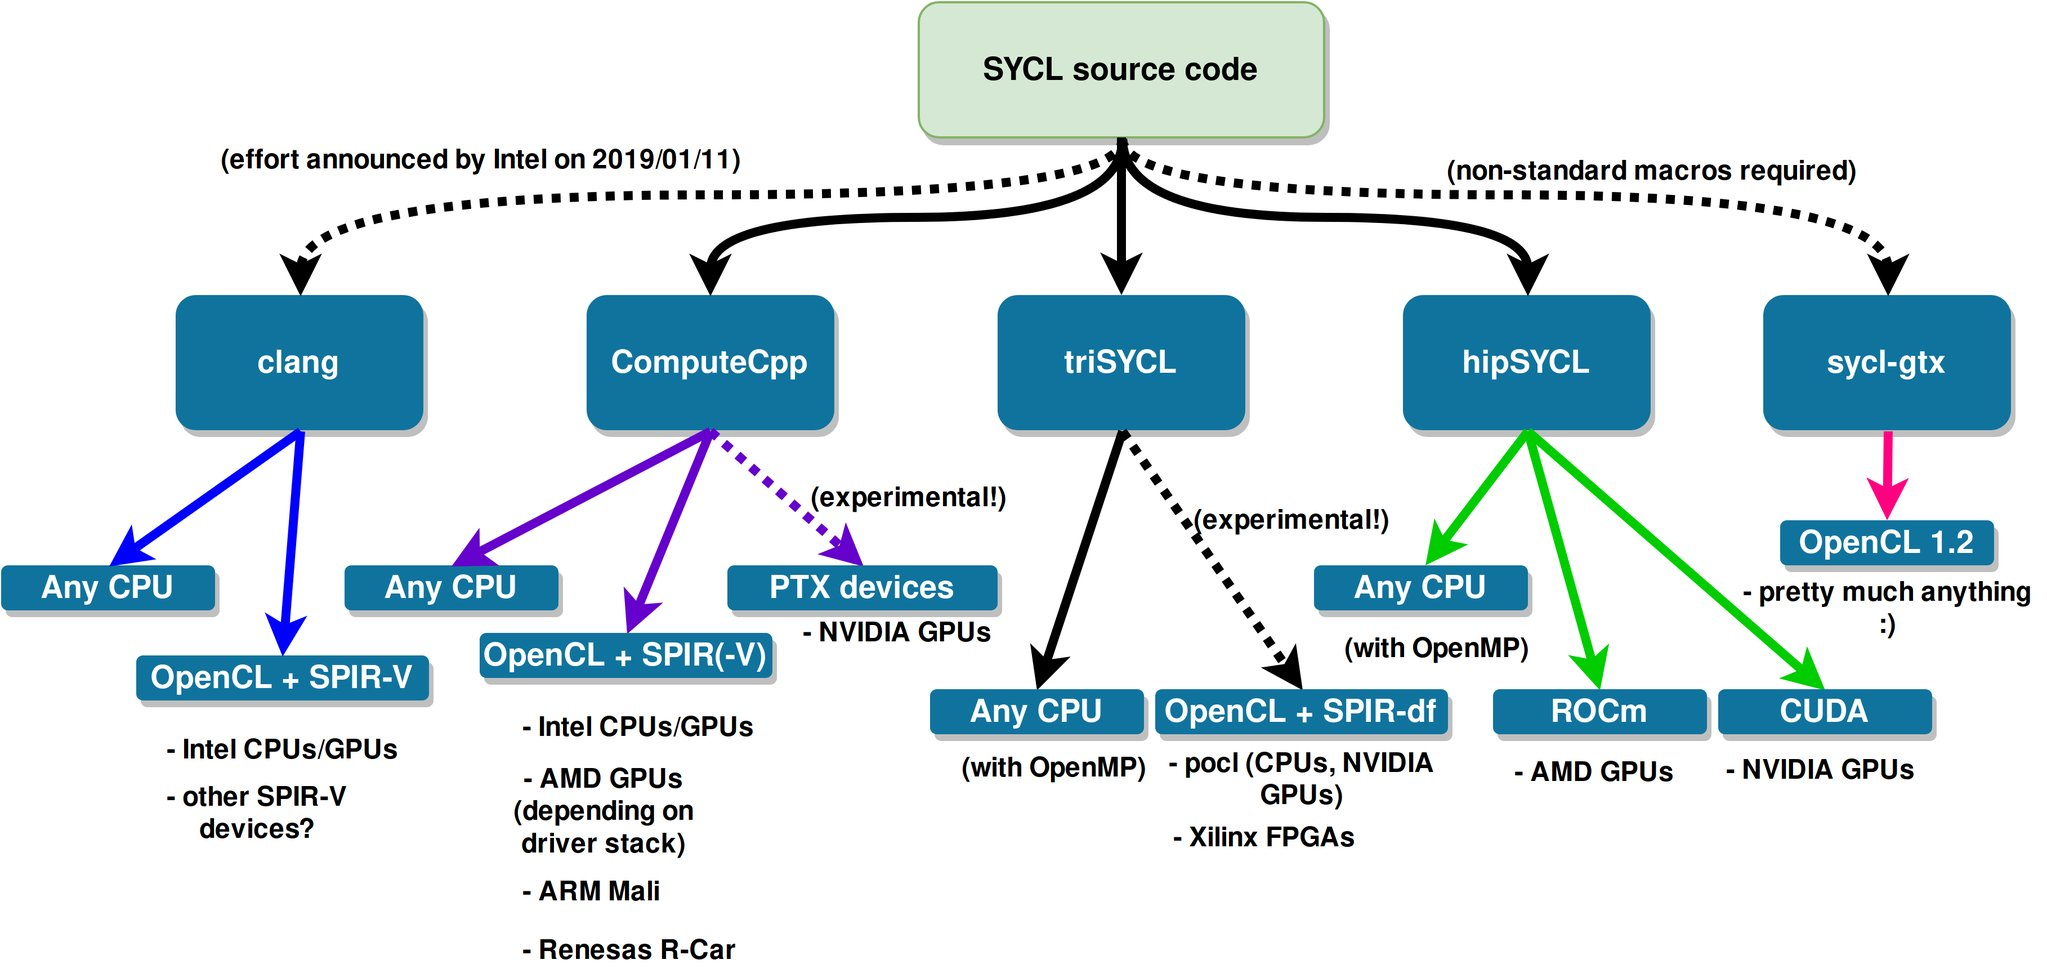
\includegraphics[width=\hsize]{Languages/SYCL/Implementations/2019-01-11-Aksel-Alpay-SYCL-implementations-DwqnsBGX4AEUZKX_jpg:large}

  Aksel Alpay 2019/01/11 \url{https://twitter.com/illuhad/status/1083863225479892993}
\end{frame}


\begin{frame}[fragile]{ComputeCpp by Codeplay}
  \url{https://www.codeplay.com/products/computesuite/computecpp}
  \begin{itemize}
  \item Codeplay is initiator \& chair of SYCL Khronos working-group
    \begin{itemize}
    \item Highly engaged in ISO C++, ADAS (MISRA \& AUTOSAR
      C++), ML, safety critical standards...
      % \begin{itemize}
      % \item Lobby all the standards, Chairing several ISO C++ WG...
      % \end{itemize}
    \item %Present at all C++ conferences
      2-day tutorial at CppCon 2019
      \url{https://www.codeplay.com/portal/08-05-19-codeplay-at-cppcon-2019-6-talks-2-workshops-and-more}
    \end{itemize}
  \item First SYCL 1.2.1 full-compliant implementation in July 2018
  \item Best implementation in class!
    \begin{itemize}
    \item Started as a developer environment for gaming (Sony PS2 \&
      PS3) in 2000's \smiley
    \item Clang/LLVM outlining compiler generating SPIR(-V) and other back-ends
    \item Runtime for OpenCL device, CPU and other back-ends (CUDA, Vulkan...)
    \end{itemize}
  \item Free community edition + non-free for customer support
    \begin{itemize}
    \item Provide several libraries \& frameworks such as SYCL
      versions of Eigen \& TensorFlow
    \end{itemize}
  %\item Probably $\approx$15 people working on SYCL environment among
  %  $\approx$70 total
  \item Implement compute \& graphics stacks for customers (Renesas,
    Imagination...)
  %\item Good company Xilinx could buy if we are interested
  %  in heterogeneous computing software! \smiley
  \end{itemize}
\end{frame}


\begin{frame}[fragile]{Clang/LLVM SYCL by Intel}
  \url{https://github.com/intel/llvm/tree/sycl}
  \begin{itemize}
  \item Open-sourced in January 2019 with unifying goal: Clang/LLVM
    up-streaming! \smiley
  \item Target CPU, GPU \& Intel FPGA
  \item Based on open-source SPIR-V LLVM translator
  \item Runtime for OpenCL
  \item Part of Intel OneAPI strategy 2018/12/12
    \url{https://www.phoronix.com/scan.php?page=news_item&px=Intel-oneAPI-Announcement}
  \item 2019/06/19 \emph{Direct programming: One API contains a new
      direct programming language, Data Parallel C++ (DPC++), an
      \alert{open, cross-industry alternative to single architecture
        proprietary languages}. DPC++ delivers parallel programming
      productivity and performance using a programming model familiar
      to developers. DPC++ is \alert{based on C++, incorporates SYCL
        from The Khronos Group and includes language extensions
        developed in an open community process}.}
    \url{https://newsroom.intel.com/news/intels-one-api-project-delivers-unified-programming-model-across-diverse-architectures}
  \end{itemize}
\end{frame}


\begin{frame}[fragile]{hipSYCL}
  \url{https://github.com/illuhad/hipSYCL}
  \begin{itemize}
  \item Started by PhD student Aksel Alpay @ Heidelberg University Computing Centre (URZ), Germany
    \begin{itemize}
    \item Around 10 developers
    \end{itemize}
  \item hipSYCL is pure single-source C++ on top of HIP and CUDA
    \begin{itemize}
    \item Interoperable with AMD ROCm \& Nvidia CUDA environments
    \item Interoperable with AMD \& Nvidia libraries \smiley
    \item Can directly use AMD \& Nvidia C++ intrinsics \smiley
      \begin{itemize}
      \item Nvidia TensorCore, Nvidia ray-tracing, graphics
        interoperability...
      \end{itemize}
    \end{itemize}
  \item Can use Clang/LLVM Cuda/HIP or \texttt{nvcc}
  \item Demonstrate that SYCL is more general than OpenCL
  \end{itemize}
\end{frame}


\begin{frame}[fragile]{triSYCL}
  \url{https://github.com/triSYCL/triSYCL}
  \begin{itemize}
  \item Open Source SYCL started in 2014 at AMD and now led by Xilinx
    \begin{itemize}
    \item Used inside Khronos to define the SYCL and OpenCL C++
      standard
      \begin{itemize}
      \item Languages are now too complex to be defined without
        implementing...
      \end{itemize}
    \end{itemize}
  \item Use C++20 templated classes
  \item OpenMP or Intel TBB for host parallelism
  \item Boost.Compute for OpenCL interaction
  \item Clang/LLVM device compiler prototype
  \item Research project targeting Xilinx FPGA and ACAP AIE CGRA
  \item Experimental fusion with Intel open-source implementation
    \url{https://github.com/triSYCL/sycl}
  \end{itemize}
\end{frame}


\section{Extensions}

\begin{frame}[fragile]{SYCL as an extensible framework}
  \begin{itemize}
  \item SYCL $\equiv$ generic heterogeneous computing model beyond OpenCL
  \item SYCL DSEL task graph model is pretty generic and not only
    OpenCL-centric
    \begin{itemize}
    \item Close to run-times such as StarPU, Nanos++, OpenAMP... and can deal
      with remote nodes, even with lower level API such as MPI,
      MCAPI...
      \begin{itemize}
      \item SYCL can target these runtimes!
      \end{itemize}
    \item Actually even not restricted to C++ either (SYPyCL, SYJaCL,
      SYJSCL, SYCaml, SYCoboL...). SYFortranCL on top of Fortran 2018?
      \smiley
    \end{itemize}
  \item Can target various accelerators, other SoC processors (ARM R5,
    Microblaze, ML...)
  \item Example in PiM (Processor-in-Memory)/Near-Memory Computing world
    \begin{itemize}
    \item Use \texttt{queue} to run on some PiM chips
    \item Use \texttt{allocator} to distribute data structures or to
      allocate \texttt{buffer} in special memory (memory page, chip...)
    \item Use \texttt{accessor} to use alternative data access (split
      address from computation, streaming only, PGAS...)
    \item Use \verb|pointer_trait| to use specific way to interact
      with memory such as bank/transposition or relocation
    \end{itemize}
  \end{itemize}
\end{frame}


\begin{frame}{Refinement levels}
  \centerline{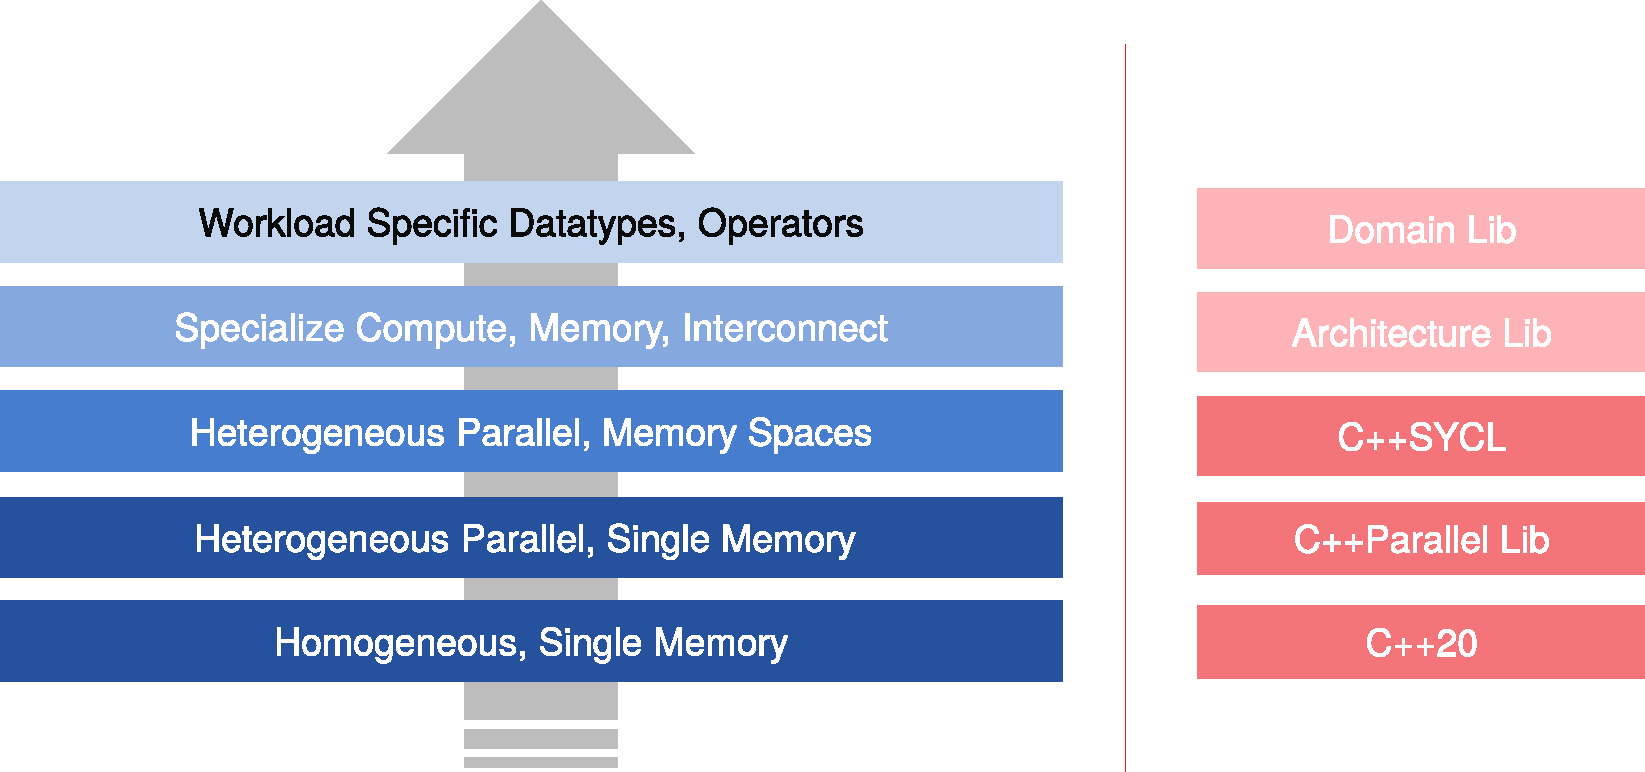
\includegraphics[height=0.9\vsize]{Languages/SYCL/refinement_levels}}
\end{frame}


\begin{frame}[fragile]{Open-source extensions as a way to speed-up standardization}
  \begin{itemize}
  \item Standardization is a slow process...
  \item Follow ISO C++ process to speed-up operations \smiley
  \item Publish and implement open-source extensions
    \begin{itemize}
    \item
      \url{https://github.com/codeplaysoftware/standards-proposals}
    \item
      \url{https://github.com/intel/llvm/tree/sycl/sycl/doc/extensions}
    \item
      \url{https://github.com/illuhad/hipSYCL/blob/master/doc/extensions.md}
    \item
      \url{https://github.com/triSYCL/triSYCL/issues?q=is%3Aissue+label%3Aextension+}
    \end{itemize}
  \item Get feedback from implementers and users \smiley
  \item Can become part of the standard if SYCL members agree
  \item Some features can be optional to allow maximum performance per
    platform
    \begin{itemize}
    \item C++ allows feature testing \& adaptability through
      metaprogramming \smiley
    \end{itemize}
  \end{itemize}
\end{frame}


\begin{frame}[fragile]{Celerity: High-level C++ for Accelerator Clusters}
  \url{https://celerity.github.io}
  \begin{itemize}
  \item Scale-out SYCL concepts at the data-center level
    \begin{itemize}
    \item Based on C++ + SYCL + MPI
    \end{itemize}
  \end{itemize}
    \begin{lstlisting}[basicstyle=\tiny]
queue.submit([=](celerity::handler& cgh) {
    auto r_input = input_buf.get_access<cl::sycl::access::mode::read>(cgh, celerity::access::neighborhood<2>(1, 1));
    auto dw_edge = edge_buf.get_access<cl::sycl::access::mode::discard_write>(cgh, celerity::access::one_to_one<2>());
    cgh.parallel_for<class MyEdgeDetectionKernel>(
        cl::sycl::range<2>(img_height - 1, img_width - 1),
        cl::sycl::id<2>(1, 1),
        [=](cl::sycl::item<2> item) {
          int sum = r_input[{item[0] + 1, item[1]}] + r_input[{item[0] - 1, item[1]}]
                  + r_input[{item[0], item[1] + 1}] + r_input[{item[0], item[1] - 1}];
          dw_edge[item] = 255 - std::max(0, sum - (4 * r_input[item]));
        }
    );
});
queue.with_master_access([=](celerity::handler& cgh) {
    auto out = edge_buf.get_access<cl::sycl::access::mode::read>(cgh, edge_buf.get_range());
    cgh.run([=]() {
        stbi_write_png("result.png", img_width, img_height, 1, out.get_pointer(), 0);
    });
});
    \end{lstlisting}
  \begin{itemize}
  \item Other C++ HPC frameworks like HPX or Kokkos provide similar
    concepts on top of SYCL but with a non-SYCL syntax
  \end{itemize}
\end{frame}


\begin{frame}[fragile]{Simplify porting code from CUDA}
  \begin{itemize}
  \item SYCL is higher-level than CUDA to ease programmer life \smiley
    \begin{itemize}
    \item Buffers for abstract storage, accessors to express
      dependencies...
    \end{itemize}
  \item But when porting CUDA code: dealing with raw device pointers,
    explicit kernel launches without any dependencies... \frownie
    \begin{itemize}
    \item Feedback from porting Eigen \& TensorFlow...
    \item \vavers Paradox: cumbersome to fit in standard SYCL model... \frownie
    \end{itemize}
  \item
    \url{https://github.com/intel/llvm/tree/sycl/sycl/doc/extensions/OrderedQueue}
    Ordered queue, in-order execution, like CUDA default stream
  \item
    \url{https://github.com/intel/llvm/blob/sycl/sycl/doc/extensions/USM}
    Unified Shared Memory like in OpenMP 5, various level of sharing
    according to hardware
  \end{itemize}
    \begin{lstlisting}[basicstyle=\scriptsize]
sycl::ordered_queue q;
auto dev = q.get_device();
auto ctxt = q.get_context();
float* a = static_cast<float*>(sycl::malloc_shared(10*sizeof(float), dev, ctxt));
float* b = static_cast<float*>(sycl::malloc_shared(10*sizeof(float), dev, ctxt));
float* c = static_cast<float*>(sycl::malloc_shared(10*sizeof(float), dev, ctxt));
q.submit([&](handler& cgh) {
  cgh.parallel_for<class vec_add>(range<1> {10}, [=](id<1> i) {
    c[i] = a[i] + b[i];
  });
});
    \end{lstlisting}
\end{frame}


\subsection{FPGA-specific features and optimizations}

\begin{frame}{Pipelining loops on FPGA}
  \begin{multicols}{2}
    \begin{itemize}
    \item Loop instructions sequentially executed by default
    \item Loop iteration starts only after last operation from
      previous iteration
    \item Elemental operations are synthesized anyway...
    \item Sequential pessimism \vavers idle hardware and loss of
      performance \frownie
    \item[\vavers] Use loop pipelining for more parallelism
    \item Efficiency measure in hardware realm: Initiation Interval
      (II)
      \begin{itemize}
      \item Clock cycles between the starting times of consecutive
        loop iterations
      \item II can be 1 if no dependency and short operations
      \end{itemize}
    \end{itemize}

    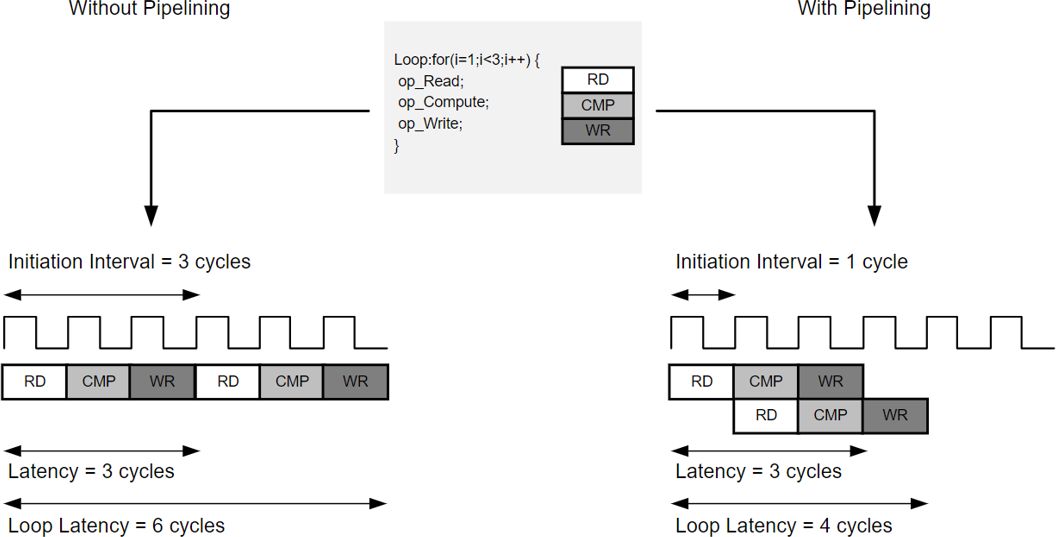
\includegraphics[width=\hsize]{Xilinx/FPGA/pipeline_execution}
  \end{multicols}
\end{frame}


\begin{frame}[fragile]{Decorating code for FPGA pipelining in triSYCL}
  \begin{multicols}{2}
    \balloon{comment}{Pipeline}{6}{6}
    \balloon{comment}{Pipeline}{10}{10}
    \begin{tikzpicture}[remember picture,overlay]
      \draw [overlay,->,very thick,red] (pic cs:PipelineS)
                                        to[bend left] (pic cs:PipelineE);
    \end{tikzpicture}
    \begin{lstlisting}[basicstyle=\scriptsize,name=Pipeline]
template<typename T, typename U>
void compute(T (&buffer_in)[BLOCK_SIZE],
             U (&buffer_out)[BLOCK_SIZE]) {
  for(int i = 0; i < NUM_ROWS; ++i) {
    for (int j = 0; j < WORD_PER_ROW; ++j) {
      vendor::xilinx::pipeline�\tikzmark{PipelineS}�([&] {
        int inTmp = buffer_in[WORD_PER_ROW*i+j];
        int outTmp = inTmp * ALPHA;
        buffer_out[WORD_PER_ROW*i+j] = outTmp;
      });
    }
  }
}
    \end{lstlisting}
    \begin{itemize}
    \item Use native C++ construct instead of alien
      \lstinline|#pragma| or attribute (vendor OpenCL or HLS
      C++\ldots)
    \item Compatible with metaprogramming
    \item Implementation
      \begin{itemize}
      \item No need for specific parser/tool-chain!
      \item Just use lambda + intrinsics! \smiley
      \end{itemize}
    \end{itemize}
    \balloono{comment}{ImplementPipeline}{5}{5}
    \begin{lstlisting}[basicstyle=\scriptsize,name=ImplementPipeline]
namespace cl::sycl::vendor::xilinx {
auto �\tikzmark{PipelineE}�pipeline = [] (auto functor) noexcept {
  /* SSDM instruction is inserted before the argument
      functor to guide xocc to do pipeline. */
  _ssdm_op_SpecPipeline(1, 1, 0, 0, "");
  functor();
};
}
    \end{lstlisting}
  \end{multicols}
\end{frame}


\begin{frame}{After Xilinx SDx \texttt{xocc}
    ingestion... Diagram in Vivado}
  \centerline{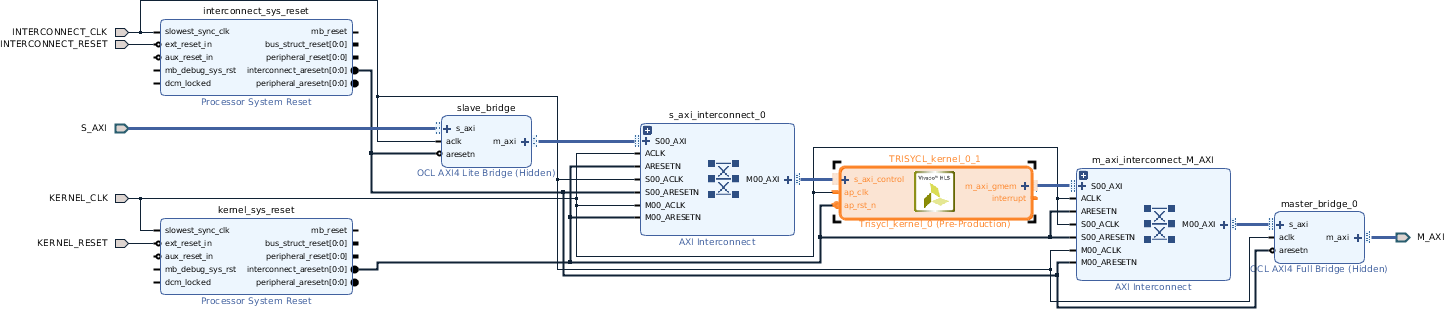
\includegraphics[width=1.1\hsize]{Images/triSYCL/triSYCL_xocc_Vivado_vector_add_diagram}}
\end{frame}


\begin{frame}{After Xilinx SDx \texttt{xocc}
    ingestion... Layout in Vivado}
  \centerline{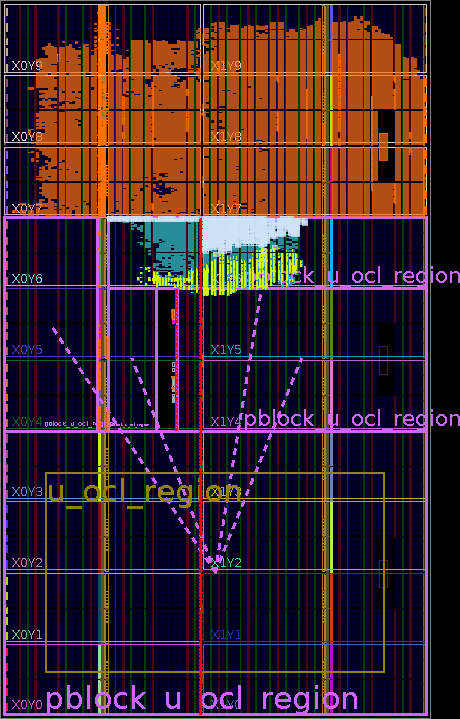
\includegraphics[height=0.9\vsize]{Images/triSYCL/triSYCL_xocc_Vivado_vector_add_layout}}
\end{frame}


\iffalse
\begin{frame}{Dataflow optimization on FPGA}
  \begin{multicols}{2}
    \begin{itemize}
    \item On CPU
      \begin{itemize}
      \item Functions are executed sequentially
      \end{itemize}
    \item On FPGA
      \begin{itemize}
      \item Functions are implemented in hardware\ldots
      \item They coexist!
      \end{itemize}
    \item Possible to execute them in parallel! \smiley
    \item Even better when in a loop
    \end{itemize}

    \includegraphics[width=\hsize]{Xilinx/FPGA/dataflow_execution}
    \begin{itemize}
    \item Dataflow execution mode
      \begin{itemize}
      \item Each function scheduled as soon as data is available
      \item Using FIFOs to forward data
      \end{itemize}
    \end{itemize}
  \end{multicols}
\end{frame}


\begin{frame}[fragile]{Decorating code for dataflow execution in triSYCL}
  \begin{multicols}{2}
    \balloon{comment}{Dataflow}{8}{8}
    \balloon{comment}{Dataflow}{12}{12}
    \begin{tikzpicture}[remember picture,overlay]
      \draw [overlay,->,very thick,red] (pic cs:DataflowS)
                                        to[bend left] (pic cs:DataflowE);
    \end{tikzpicture}
    \begin{lstlisting}[basicstyle=\scriptsize,name=Dataflow]
cgh.single_task<class add>(
  [=,
   d_a = drt::accessor<decltype(a_a)> { a_a },
   d_b = drt::accessor<decltype(a_b)> { a_b }
   ] {
    int buffer_in[BLOCK_SIZE];
    int buffer_out[BLOCK_SIZE];
    vendor::xilinx::dataflow�\tikzmark{DataflowS}�([&] {
        readInput(buffer_in, d_b);
        compute(buffer_in, buffer_out);
        writeOutput(buffer_out, d_a);
      });
  });
    \end{lstlisting}
    \begin{itemize}
    \item Use native C++ construct instead of alien
      \lstinline|#pragma| or attribute (vendor OpenCL or HLS
      C++\ldots)
    \item Compatible with metaprogramming
    \item Implementation
      \begin{itemize}
      \item No need for specific parser/tool-chain!
      \item Just use lambda + intrinsics! \smiley
      \end{itemize}
    \end{itemize}
    \balloono{comment}{ImplementDataflow}{5}{5}
    \begin{lstlisting}[basicstyle=\scriptsize,name=ImplementDataflow]
namespace cl::sycl::vendor::xilinx {
auto �\tikzmark{DataflowE}�dataflow = [] (auto functor) noexcept {
  /* SSDM instruction is inserted before the argument
     functor to guide xocc to do dataflow. */
  _ssdm_op_SpecDataflowPipeline(-1, "");
  functor();
};
}
    \end{lstlisting}
  \end{multicols}
\end{frame}

\fi

\begin{trans}{Partitioning memories}
  \begin{multicols}{2}
    \begin{itemize}
    \item Remember memory bank conflicts on Cray vector computers in
      the 70's?
    \item In FPGA world, even memory is configurable!
    \item Example of array with 16 elements\ldots
    \item Cyclic Partitioning
      \begin{itemize}
      \item Each array element distributed to physical memory
        banks in order and cyclically
      \item Banks accessed in parallel \vavers improved bandwidth
      \item Reduce latency for pipelined sequential accesses
      \end{itemize}
    \end{itemize}
    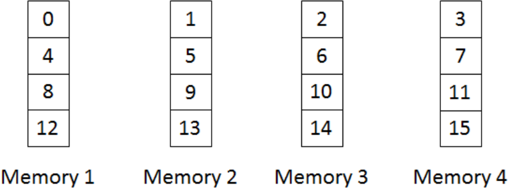
\includegraphics[width=\hsize]{Xilinx/FPGA/cyclic_partition_array}
  \end{multicols}

  \begin{multicols}{2}
    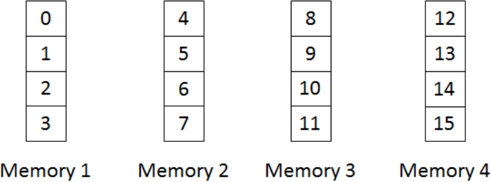
\includegraphics[width=\hsize]{Xilinx/FPGA/block_partition_array}
    \begin{itemize}
    \item Block Partitioning
      \begin{itemize}
      \item Each array element distributed to physical memory banks by
        block and in order
      \item Banks accessed in parallel \vavers improved bandwidth
      \item Reduce latency for pipelined accesses with some
        distribution
      \end{itemize}
    \item Complete Partitioning
      \begin{itemize}
      \item Extreme distribution
      \item Extreme bandwidth
      \item Low latency
      \end{itemize}
    \end{itemize}
    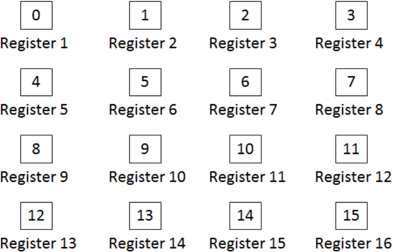
\includegraphics[width=\hsize]{Xilinx/FPGA/complete_partition_array}
  \end{multicols}
\end{trans}


\begin{trans}{\texttt{partition\_array} class in triSYCL use case}
  Enhanced \lstinline|std::array|
  \begin{multicols}{2}
    \begin{lstlisting}[basicstyle=\scriptsize,name=PartitionSYCL]
cgh.single_task<class add>([=] {
  // Cyclic partition for A as matrix
  // multiplication needs row-wise
  // parallel access
  xilinx::partition_array<Type, BLOCK_SIZE,
    xilinx::partition::cyclic<MAX_DIM>> A;
  // Block partition for B as matrix
  // multiplication needs column-wise
  // parallel access
  xilinx::partition_array<Type, BLOCK_SIZE,
    xilinx::partition::block<MAX_DIM>> B;
  xilinx::partition_array<Type, BLOCK_SIZE> C;
  [...]
});
    \end{lstlisting}
    \columnbreak
    \begin{itemize}
    \item Xilinx Vivado HLS C++
      \begin{lstlisting}[basicstyle=\scriptsize,name=PartitionHLS]
int A[MAX_DIM * MAX_DIM];
int B[MAX_DIM * MAX_DIM];
int C[MAX_DIM * MAX_DIM];
#pragma HLS ARRAY_PARTITION variable=A dim=1 \
                            cyclic factor=64
#pragma HLS ARRAY_PARTITION variable=B dim=1 \
                            block factor=64
      \end{lstlisting}
    \item Xilinx SDx OpenCL C
      \begin{lstlisting}[basicstyle=\scriptsize,name=PartitionOpenCL]
int A[MAX_DIM * MAX_DIM]
__attribute__((xcl_array_partition
               (cyclic, MAX_DIM, 1)));
int B[MAX_DIM * MAX_DIM]
__attribute__((xcl_array_partition
               (block, MAX_DIM, 1)));
int C[MAX_DIM * MAX_DIM];
      \end{lstlisting}
    \end{itemize}
  \end{multicols}
\end{trans}


\iffalse

\begin{frame}{Effect of array block and cyclic partitioning on matrix
    multiplication}
  \centerline{\includegraphics[height=0.8\vsize]{triSYCL/Results-2018-02/array_partition_kernel_exe_time}}
  \textbf{a}: array partitioning, \textbf{p}: pipelining, \textbf{no
    opt}: non optimized (but \texttt{-O3} triSYCL)
\end{frame}


\begin{frame}{Single-source brings more optimization}
  \begin{itemize}
  \item Kernel code optimized according to host parameter value or
    data type
    \begin{itemize}
    \item A host constant scalar can be inlined into the kernel
      \begin{itemize}
      \item Save one API call to send the parameter to the kernel
      \end{itemize}
    \item A host constant array/tensor can be inlined into the kernel
      \begin{itemize}
      \item Save one API call to send the parameter to the kernel
      \item Replace memory access by direct constant computation
      \end{itemize}
    \item Dead-code elimination
    \item \ldots
    \end{itemize}
  \item Single-source allows kernel fusion with (manual) metaprogramming
    \begin{itemize}
    \item Kernel fusion heavily used in TensorFlow for example
    \item Kernel fusion leads to better performance by reducing the
      launch \& memory overhead
    \end{itemize}
  \item[\vavers] Can lead to better performance compared to
    split-source (OpenCL, HLS C/C++\ldots)
  \end{itemize}
\end{frame}

\fi

\subsection{Coarse Grain Configurable Array (CGRA)}


\begin{frame}{Xilinx C++ ACAP: templated 2D SYCL abstractions}
  \centerline{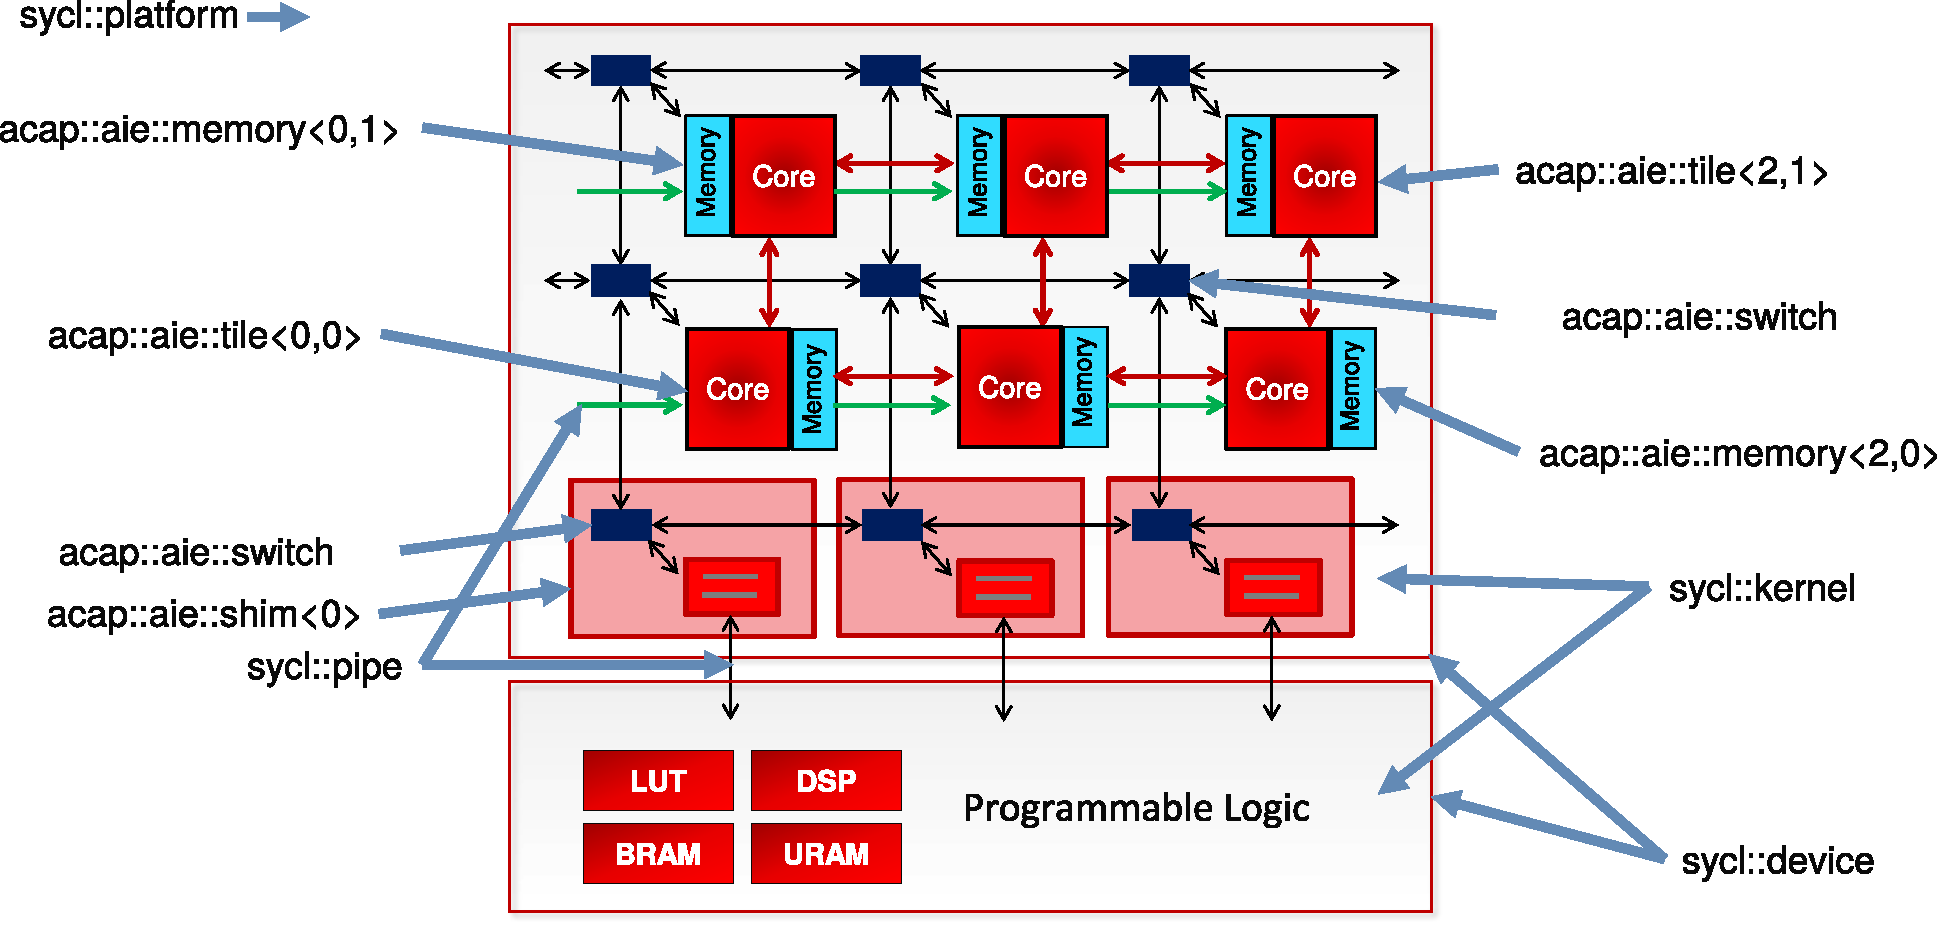
\includegraphics[height=0.9\vsize]{Languages/SYCL/ACAP/ACAP_templated_2D_abstractions}}
\end{frame}


\begin{frame}{C++ ACAP abstractions for the ultra-performance programmer}
  \begin{itemize}
  \item Executable DSEL in modern C++
    \begin{itemize}
    \item Allows debug with CPU tools on laptop (ThreadSanitizer,
      Valgrind, GDB....)
    \item Allow architecture co-design before silicon. No need for
      expensive RTL emulator/simulator to start with \smiley
    \end{itemize}
  \item 2D layout and connectivity
  \item AIE cores
  \item Memory modules
    \begin{itemize}
    \item Banks
    \item Locking units
    \end{itemize}
  \item DMA
  \item Cascade stream
  \item Routing resource
    \begin{itemize}
    \item Virtual circuit \& packet switching
    \item Routing tables \& broadcast mode
    \end{itemize}
    Interconnection with FPGA programmable logic (PL), GPU, host...
  \item Events I/O \& configuration/modes
  \end{itemize}
\end{frame}


\section{Conclusion}

\begin{frame}[fragile]{Resources}
  \begin{itemize}
  \item \url{https://www.khronos.org/sycl}
    \begin{itemize}
    \item
      \url{https://www.khronos.org/files/sycl/sycl-121-reference-card.pdf}
      8 pages of SYCL \&
    \end{itemize}
  \item \url{https://sycl.tech} community content
  \item
    \url{https://tech.io/playgrounds/48226/introduction-to-sycl/introduction-to-sycl-2}
    playground on ``Introduction to SYCL'' with on-line code execution
  \item Code samples from Codeplay
    \url{https://github.com/codeplaysoftware/computecpp-sdk/tree/master/samples}
  \item Parallel Research Kernels implemented with different
    frameworks, including SYCL
    \begin{itemize}
    \item Useful to compare or translate between different programming
      models
    \item \url{https://github.com/ParRes/Kernels}
    \end{itemize}
  \end{itemize}
\end{frame}


\begin{frame}{Puns and pronunciation explained}
  \begin{center}
    \begin{tabular}[c]{c}
      SYCL\\
      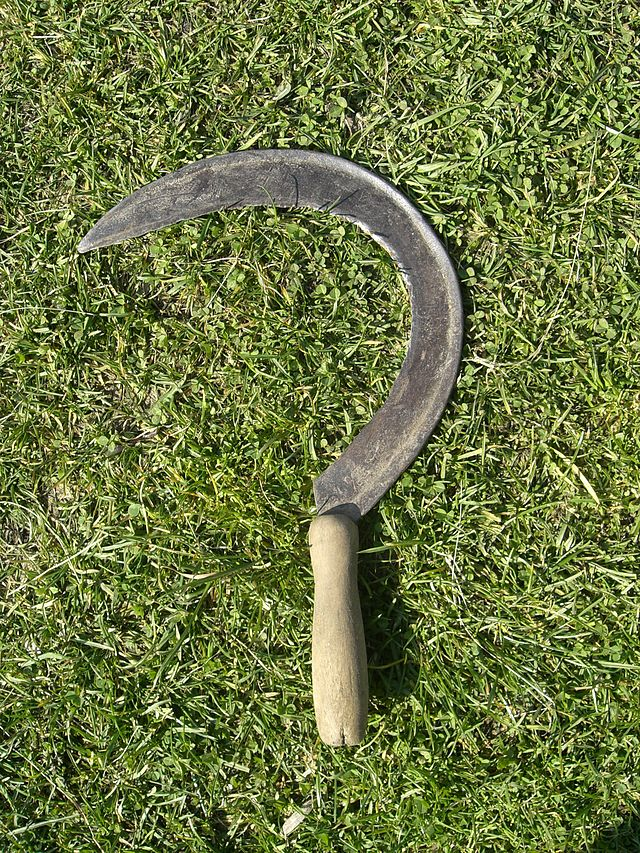
\includegraphics[height=0.7\vsize]{Pictures/Sickle33}\\
      sickle [ \textprimstress si-k\textschwa l ]
    \end{tabular}
    \begin{tabular}[c]{c}
      SPIR\\
      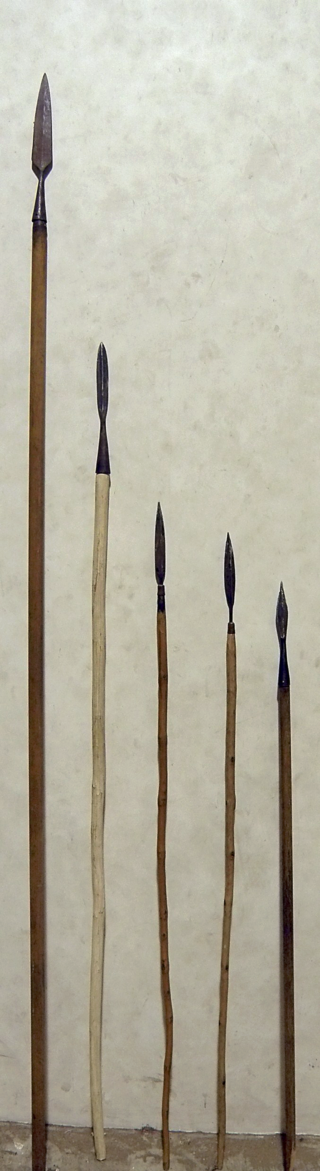
\includegraphics[height=0.7\vsize]{Pictures/A_spear_and_a_series_of_javelins}\\
      spear [ \textprimstress spir ]
    \end{tabular}
  \end{center}
\end{frame}


\begin{frame}{SYCL mascot: SYCL the seagull!}
  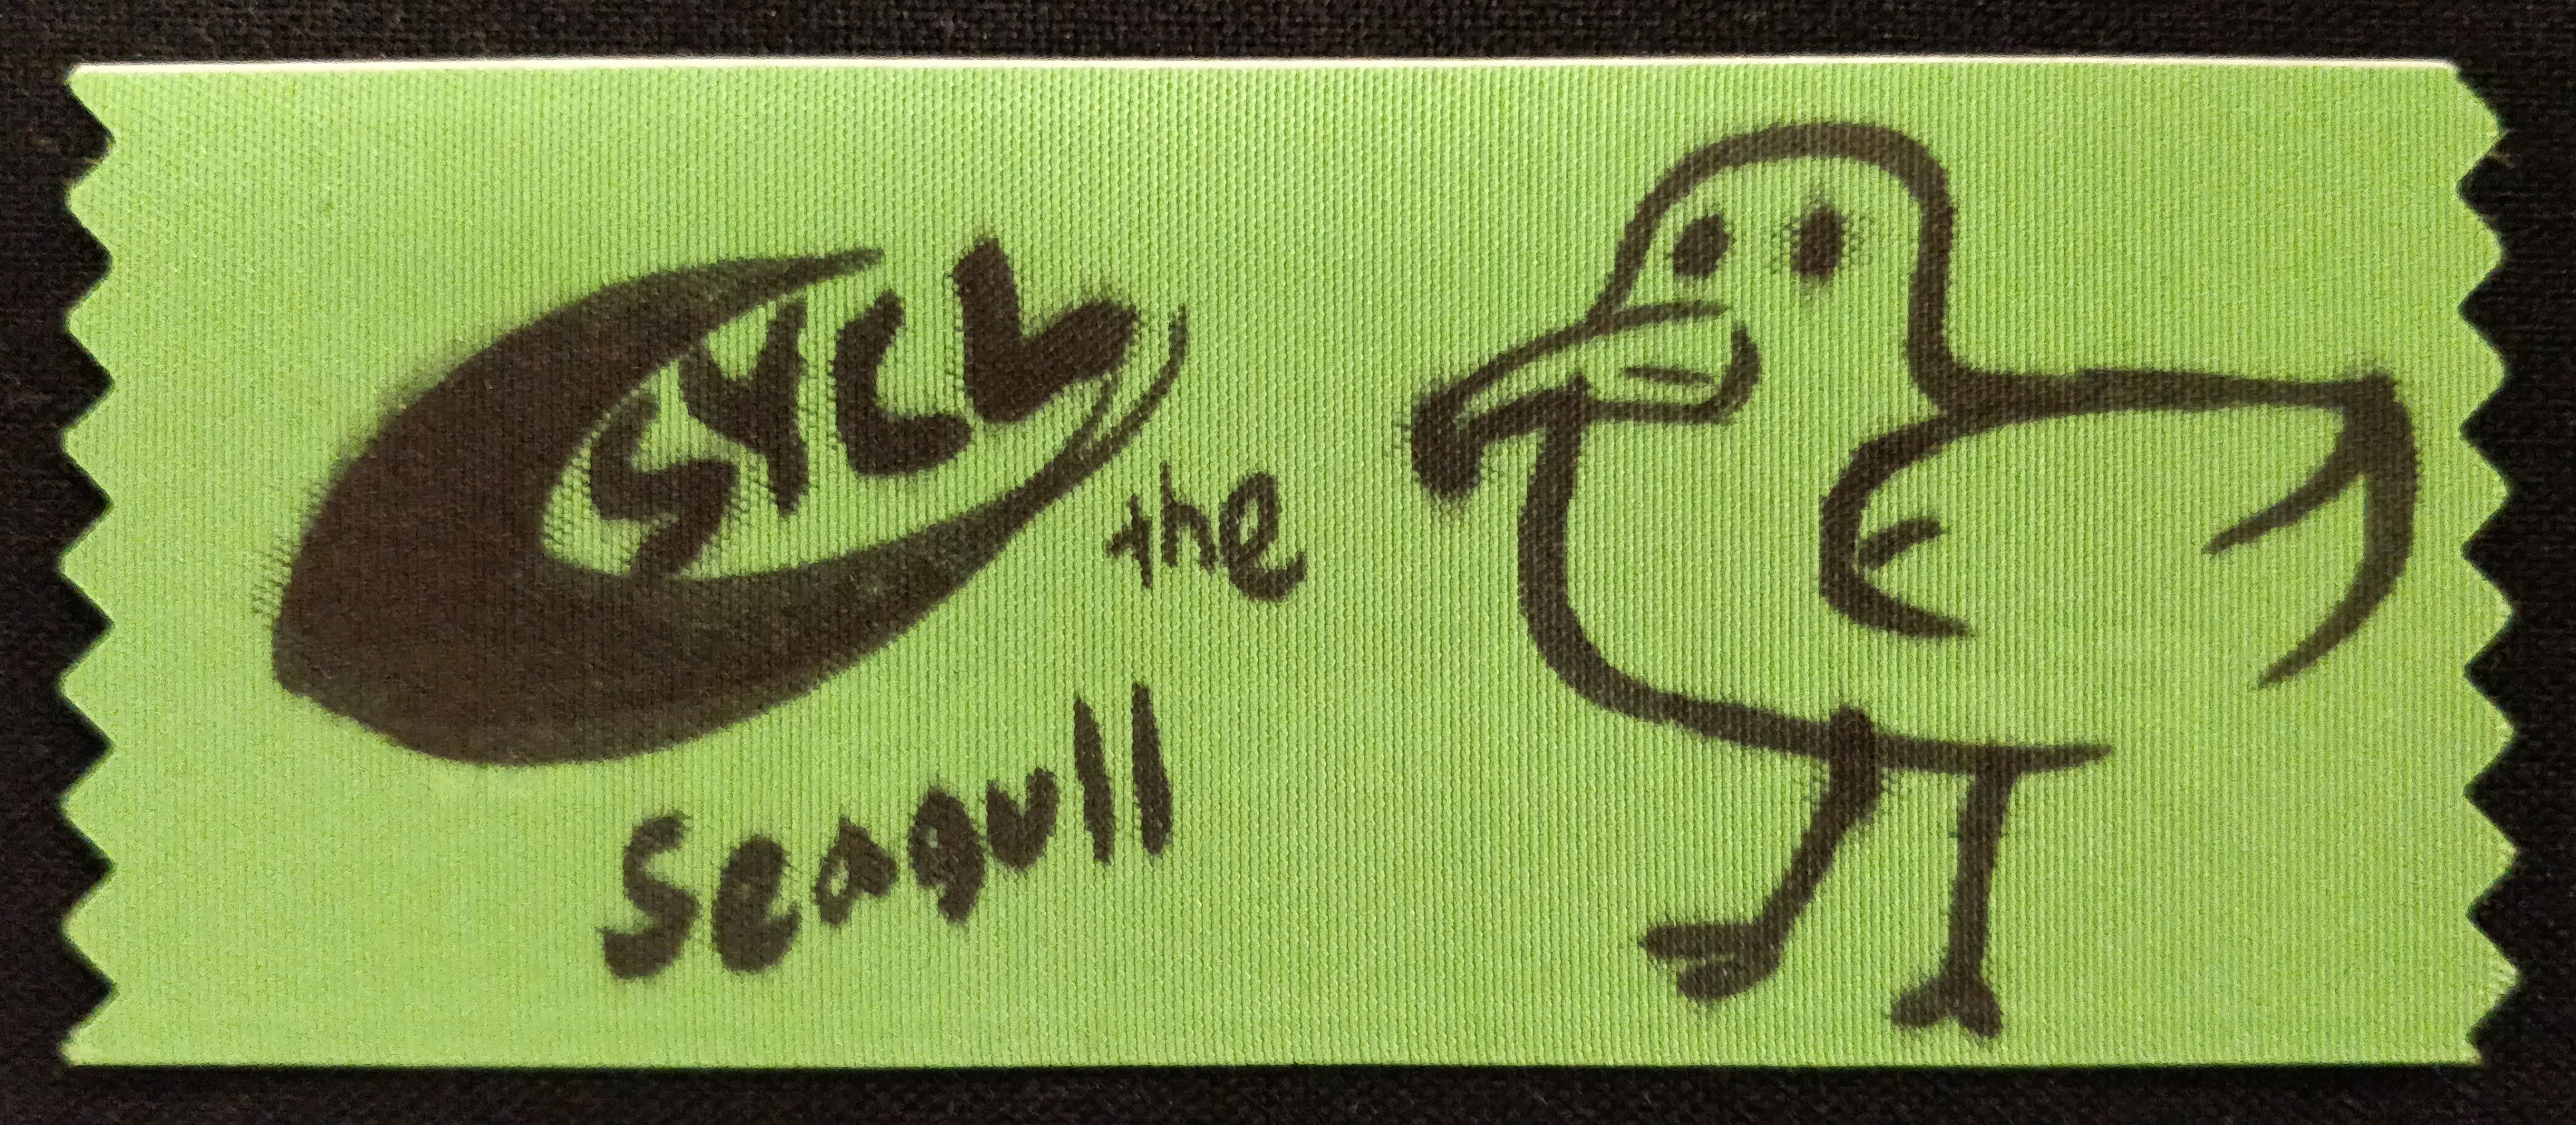
\includegraphics[width=\hsize]{Languages/SYCL/Mascot/SYCL_the_Seagull}

  Thanks to Dominic Agoro-Ombaka during Khronos face-to-face meeting
  in Montr�al !
\end{frame}


\begin{frame}[fragile]{Conclusion}
  \begin{itemize}
  \item Heterogeneous computing is everywhere and here to stay
    \begin{itemize}
    \item \emph{``The next decade will see a Cambrian explosion of novel computer
      architectures''}
    \item Full systems \& HPC machines add other complexity levels...
    \end{itemize}
  \item SYCL C++ standard from Khronos Group
    \begin{itemize}
    \item In post-modern C++ we trust: only way to control the full
      stack of real hardware. It's not magic, it's C++! \smiley
    \item Pure modern C++ DSEL for heterogeneous computing
    \item Single-source \& single-language to metaprogram the full
      architecture
    \item ISO C++ is an elitist democracy: only what is implemented
      and working is ratified
      \begin{itemize}
      \item SYCL implementations \vavers feedback for ISO C++
        WG21 SG14 standard...
      \end{itemize}
    \end{itemize}
  \item Open-source + open standards
    \begin{itemize}
    \item No user locked-in!
    \item Various implementation with various back-ends
    \item Interoperability with other ecosystems (OpenCL, CUDA,
      Vulkan, proprietary...)
    \end{itemize}
  \item You are not happy? Do it the standard way! Participate to the
    standards to have a real impact! \smiley
  \end{itemize}
\end{frame}


\section*{Table of content}

\begin{multicols}{2}
  \tiny
  \tableofcontents[frametitles]
  \textbf{You are here      !}\hfill\expandafter\the\csname c@page\endcsname
\end{multicols}


\end{document}


%%% Local Variables:
%%% mode: latex
%%% ispell-local-dictionary: "american"
%%% TeX-auto-untabify: t
%%% TeX-PDF-mode: t
%%% TeX-master: t
%%% End:

% vim:spell spelllang=en
